
\ifdefined\ishandout
\documentclass[11pt,english,handout]{beamer}
\else
\documentclass[11pt,english]{beamer}
\fi

%\documentclass[11pt]{beamer}
\usepackage{mathptmx}
\renewcommand{\sfdefault}{lmss}
\renewcommand{\familydefault}{\sfdefault}
\usepackage[T1]{fontenc}
\usepackage[latin9]{inputenc}
\usepackage{amsmath}
\usepackage{amssymb}
\usepackage{graphicx}
\PassOptionsToPackage{normalem}{ulem}
\usepackage{ulem}
\usepackage{caption}
\captionsetup{labelformat=empty}
\usepackage{bbm}
\usepackage{upgreek}
\usepackage{graphicx}
\setbeamertemplate{section in toc}[sections numbered]
\makeatletter
\usepackage{caption} 
\captionsetup[table]{skip=10pt}
%%%%%%%%%%%%%%%%%%%%%%%%%%%%%% Textclass specific LaTeX commands.
% this default might be overridden by plain title style
\newcommand\makebeamertitle{\frame{\maketitle}}%
% (ERT) argument for the TOC
\AtBeginDocument{%
	\let\origtableofcontents=\tableofcontents
	\def\tableofcontents{\@ifnextchar[{\origtableofcontents}{\gobbletableofcontents}}
	\def\gobbletableofcontents#1{\origtableofcontents}
}

%%%%%%%%%%%%%%%%%%%%%%%%%%%%%% User specified LaTeX commands.
%\documentclass[presentation]{beamer}


\def\Tiny{\fontsize{7pt}{8pt}\selectfont}
\def\Normal{\fontsize{8pt}{10pt}\selectfont}

\usetheme{Madrid}
\usecolortheme{lily}
%\setbeamercovered{transparent}
\useinnertheme{rounded}


\setbeamertemplate{footline}{\hfill\Normal{\insertframenumber/\inserttotalframenumber}}
%\setbeamertemplate{footline}{}

\setbeamertemplate{navigation symbols}{}

\newenvironment{changemargin}[2]{%
	\begin{list}{}{%
			\setlength{\topsep}{0pt}%
			\setlength{\leftmargin}{#1}%
			\setlength{\rightmargin}{#2}%
			\setlength{\listparindent}{\parindent}%
			\setlength{\itemindent}{\parindent}%
			\setlength{\parsep}{\parskip}% 
		}%
		\item[]}{\end{list}}

\setbeamertemplate{footline}{\hfill\insertframenumber/\inserttotalframenumber}
\setbeamertemplate{navigation symbols}{}

%\usepackage{times}  % fonts are up to you
\usepackage{graphicx}
%\usepackage{graphics}
\usepackage{epsfig}
\usepackage{bm}
\usepackage{epsf}
\usepackage{float}
\usepackage[final]{pdfpages}
\usepackage{multirow}
\usepackage{colortbl}
\usepackage{xkeyval}
%\usepackage{sgame}
%\usepackage{pst-node}
\usepackage{listings}
\usepackage{ifthen}
%\usepackage{hyperref}
\usepackage{tikz}

%\usepackage{times}  % fonts are up to you
%\usepackage{graphicx}
%\usepackage{graphics}
\usepackage{epsfig,bm,epsf,float}
\usepackage[final]{pdfpages}
\usepackage{xcolor,multirow,colortbl}
\usepackage{xkeyval}
\usepackage{verbatim}
%\usepackage{sgame}
%\usepackage{pst-node}
\usepackage{listings}
%\usepackage{handoutWithNotes}
%\pgfpagesuselayout{3 on 1 with notes}[letterpaper,border shrink=5mm]
%\pgfpagesuselayout{2 on 1 with notes landscape}[letterpaper,border shrink=5mm]
\usepackage{setspace}
\usepackage{ragged2e}

\setbeamersize{text margin left=1em,text margin right=1em} % CambridgeUS spacing if you use default instead


%\pdfmapfile{+sansmathaccent.map}

% Table formatting
\usepackage{booktabs}


% Decimal align
\usepackage{dcolumn}
\newcolumntype{d}[0]{D{.}{.}{5}}


\global\long\def\expec#1{\mathbb{E}\left[#1\right]}
\global\long\def\var#1{\mathrm{Var}\left[#1\right]}
\global\long\def\cov#1{\mathrm{Cov}\left[#1\right]}
\global\long\def\prob#1{\mathrm{Prob}\left[#1\right]}
\global\long\def\one{\mathbf{1}}
\global\long\def\diag{\operatorname{diag}}
\global\long\def\expe#1#2{\mathbb{E}_{#1}\left[#2\right]}
\DeclareMathOperator*{\plim}{\text{plim}}

%\usefonttheme[onlymath]{serif}

\usepackage{appendixnumberbeamer}
\renewcommand{\thefootnote}{}

\setbeamertemplate{footline}
{
	\leavevmode%
	%   \hbox{%
	%      \begin{beamercolorbox}[wd=\paperwidth,ht=2.25ex,dp=1ex,right]{date in head/foot}%
	%\usebeamerfont{date in head/foot}\insertshortdate{}\hspace*{2em}%
	\hfill
	%turning the next line into a comment, erases the frame numbers
	\insertframenumber{}\hspace*{2ex}\vspace{1ex}
	
	%    \end{beamercolorbox}}%
}

\definecolor{blue}{RGB}{0, 0, 210}
\definecolor{red}{RGB}{170, 0, 0}

\makeatother

\usepackage[english]{babel}

\usepackage{tikz}
\newcommand*\circled[1]{\tikz[baseline=(char.base)]{             \node[circle,ball color=structure.fg, shade,   color=white,inner sep=1.2pt] (char) {\tiny #1};}} 

\makeatletter
\let\save@measuring@true\measuring@true
\def\measuring@true{%
	\save@measuring@true
	\def\beamer@sortzero##1{\beamer@ifnextcharospec{\beamer@sortzeroread{##1}}{}}%
	\def\beamer@sortzeroread##1<##2>{}%
	\def\beamer@finalnospec{}%
}
\makeatother



\setbeamersize{text margin left= .8em,text margin right=1em} 
\newenvironment{wideitemize}{\itemize\addtolength{\itemsep}{10pt}}{\enditemize}
\newenvironment{wideitemizeshort}{\itemize}{\enditemize}

\newcommand{\indep}{\perp\!\!\!\!\perp} 

\begin{document}
	
	%% Title slide
	\begin{frame}[noframenumbering]{}
		\vspace{0.5cm}
		\title[]{Chapter 4: Introduction to Regression}
		\author{Jonathan Roth}
		\date{Mathematical Econometrics I \\ Brown University\\Fall 2023} 
		\titlepage {\small{}\ }\thispagestyle{empty} \vspace{-30pt}
		
	\end{frame}

	
\begin{frame} {Motivation}

\begin{wideitemize}

\item
We showed that under conditional unconfoundedness we can learn the conditional average treatment effect (CATE) by comparing outcome means for the treatment/control group conditional on $X_i$:
$$ CATE(x) = E[ Y_i | D_i = 1 , X_i = x ] - E[Y_i | D_i = 0 ,X_i =x ]$$ 

\item
When $X_i$ is discrete and we have many observations per $x$-value ($N_x$ is large), we showed how we can use the Central Limit Theorem to estimate each of these conditional means and ``do inference'' 

\pause
\item
But what about when $X_i$ is continuous?

\end{wideitemize}
	
\end{frame}	


\begin{frame}
\centering

\only<1-7>{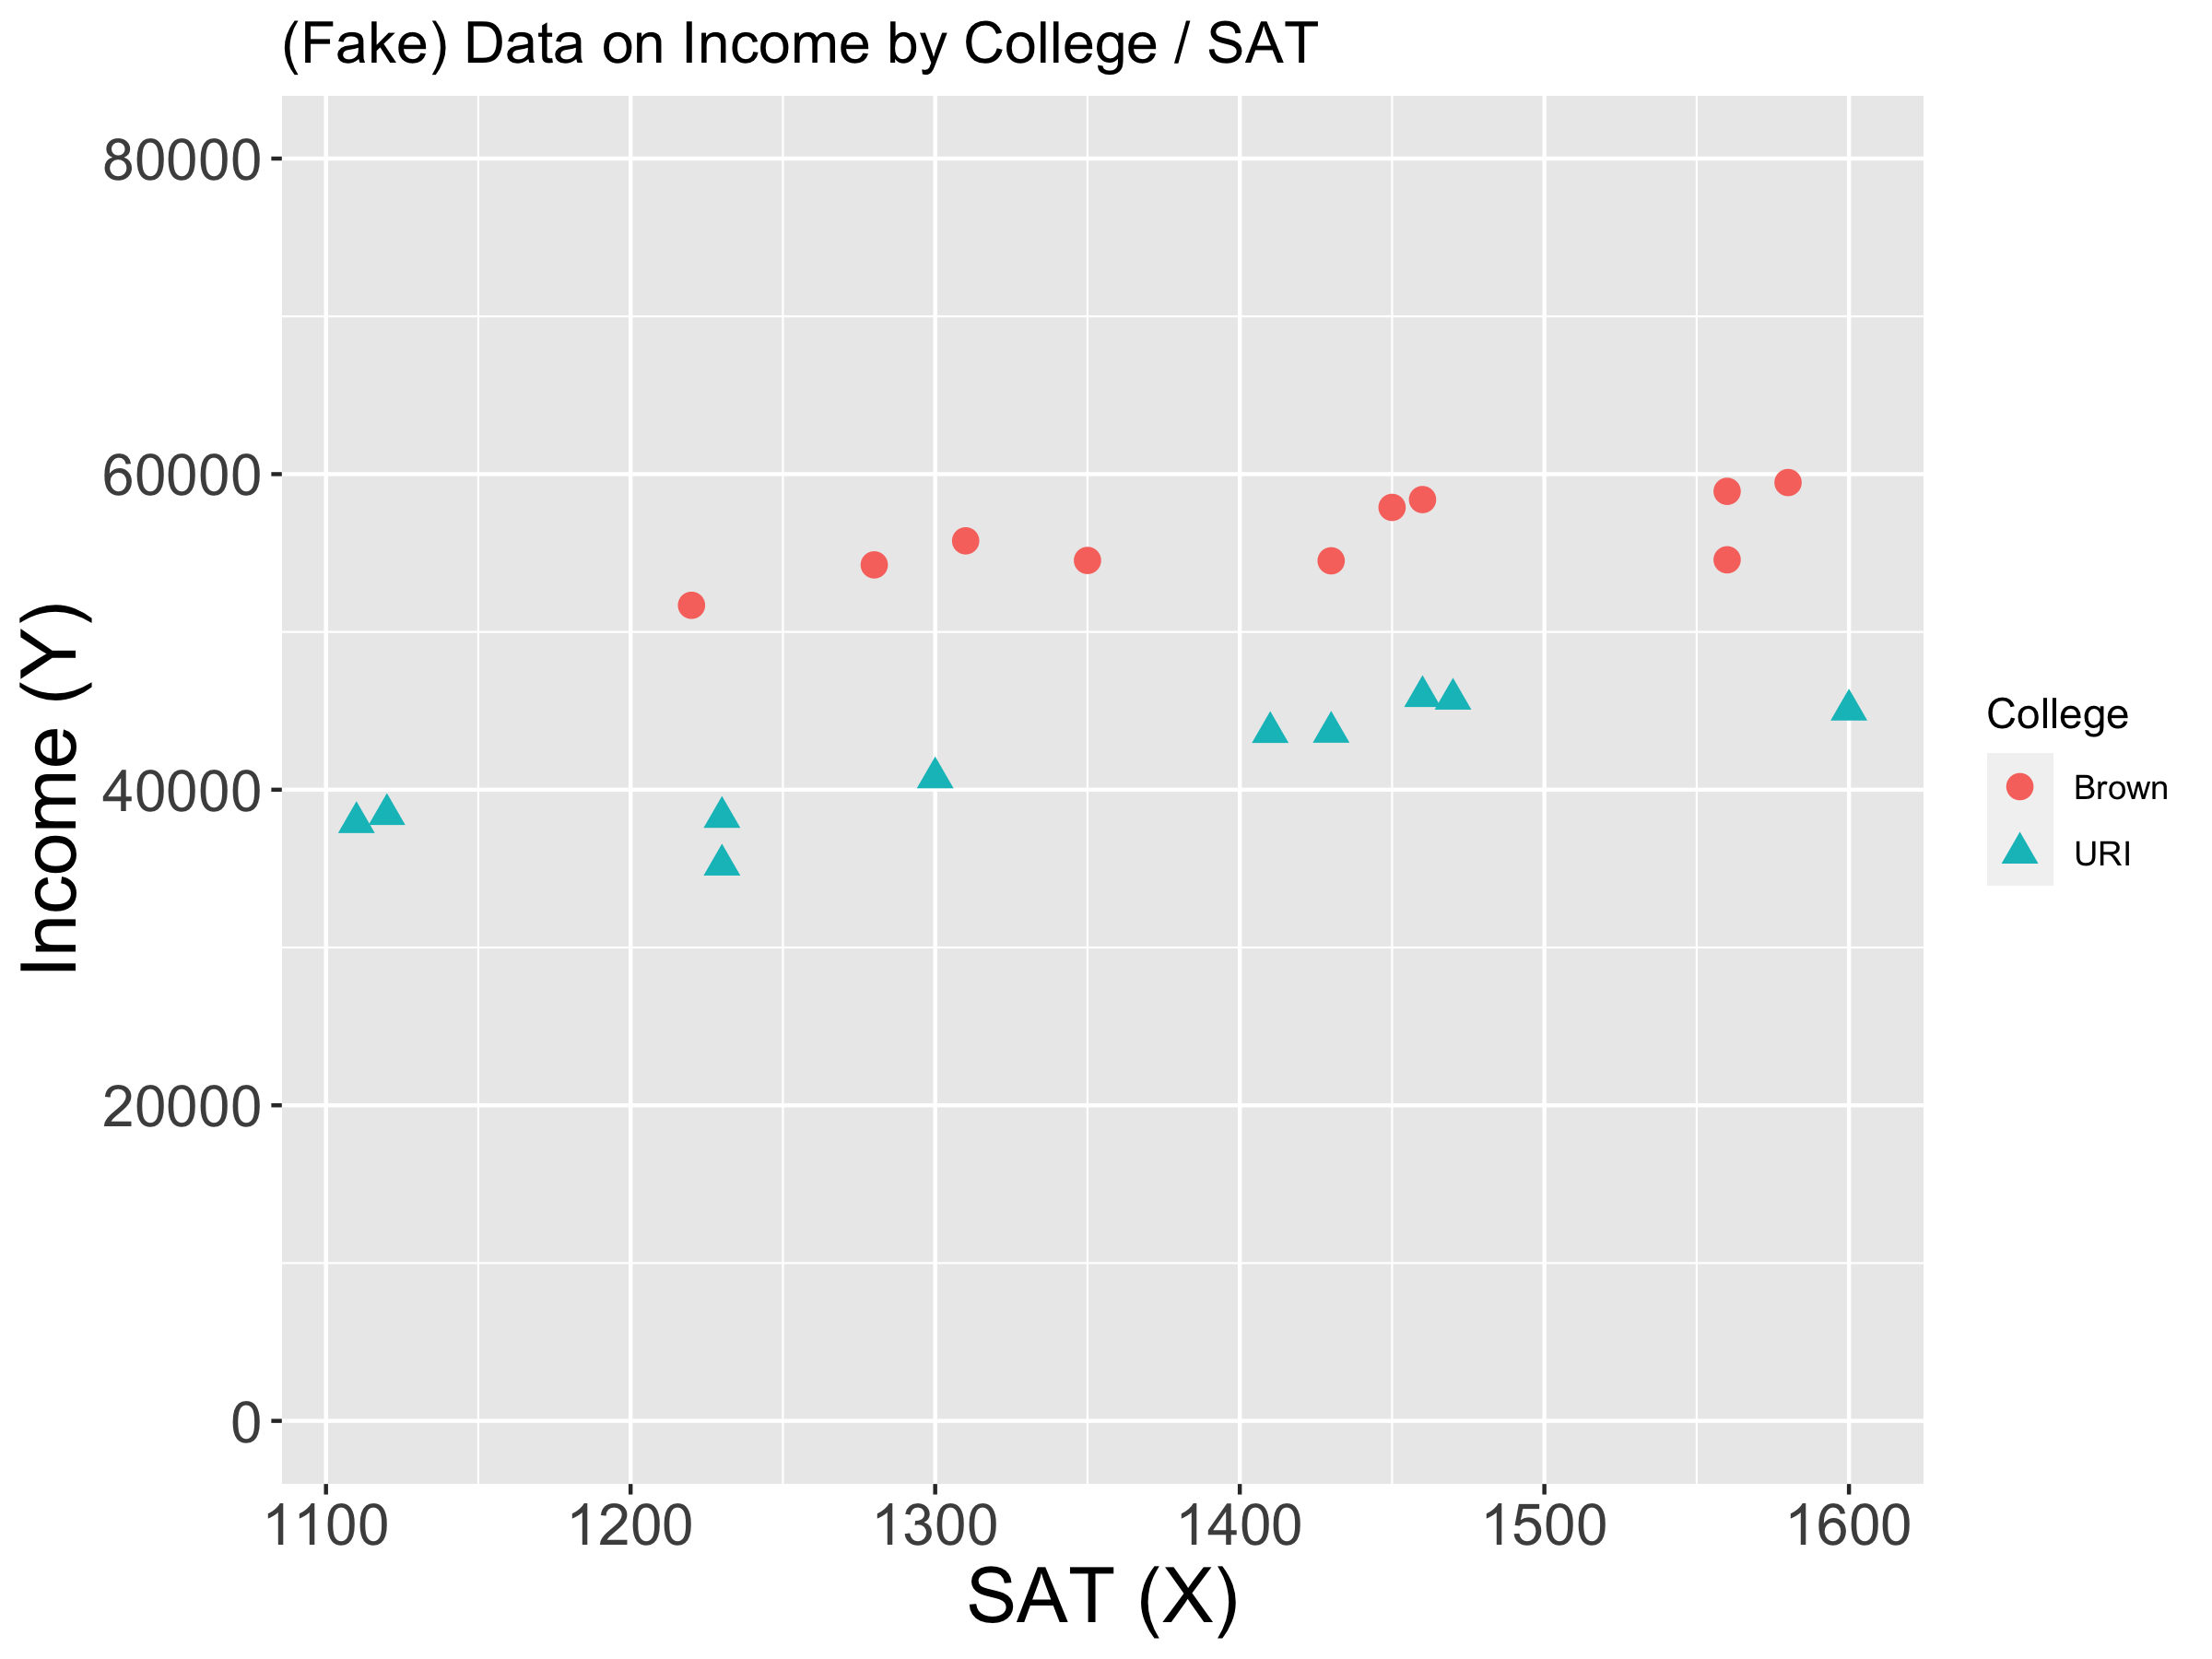
\includegraphics[width = 0.8 \linewidth]{fake-sat.png}}
\only<8>{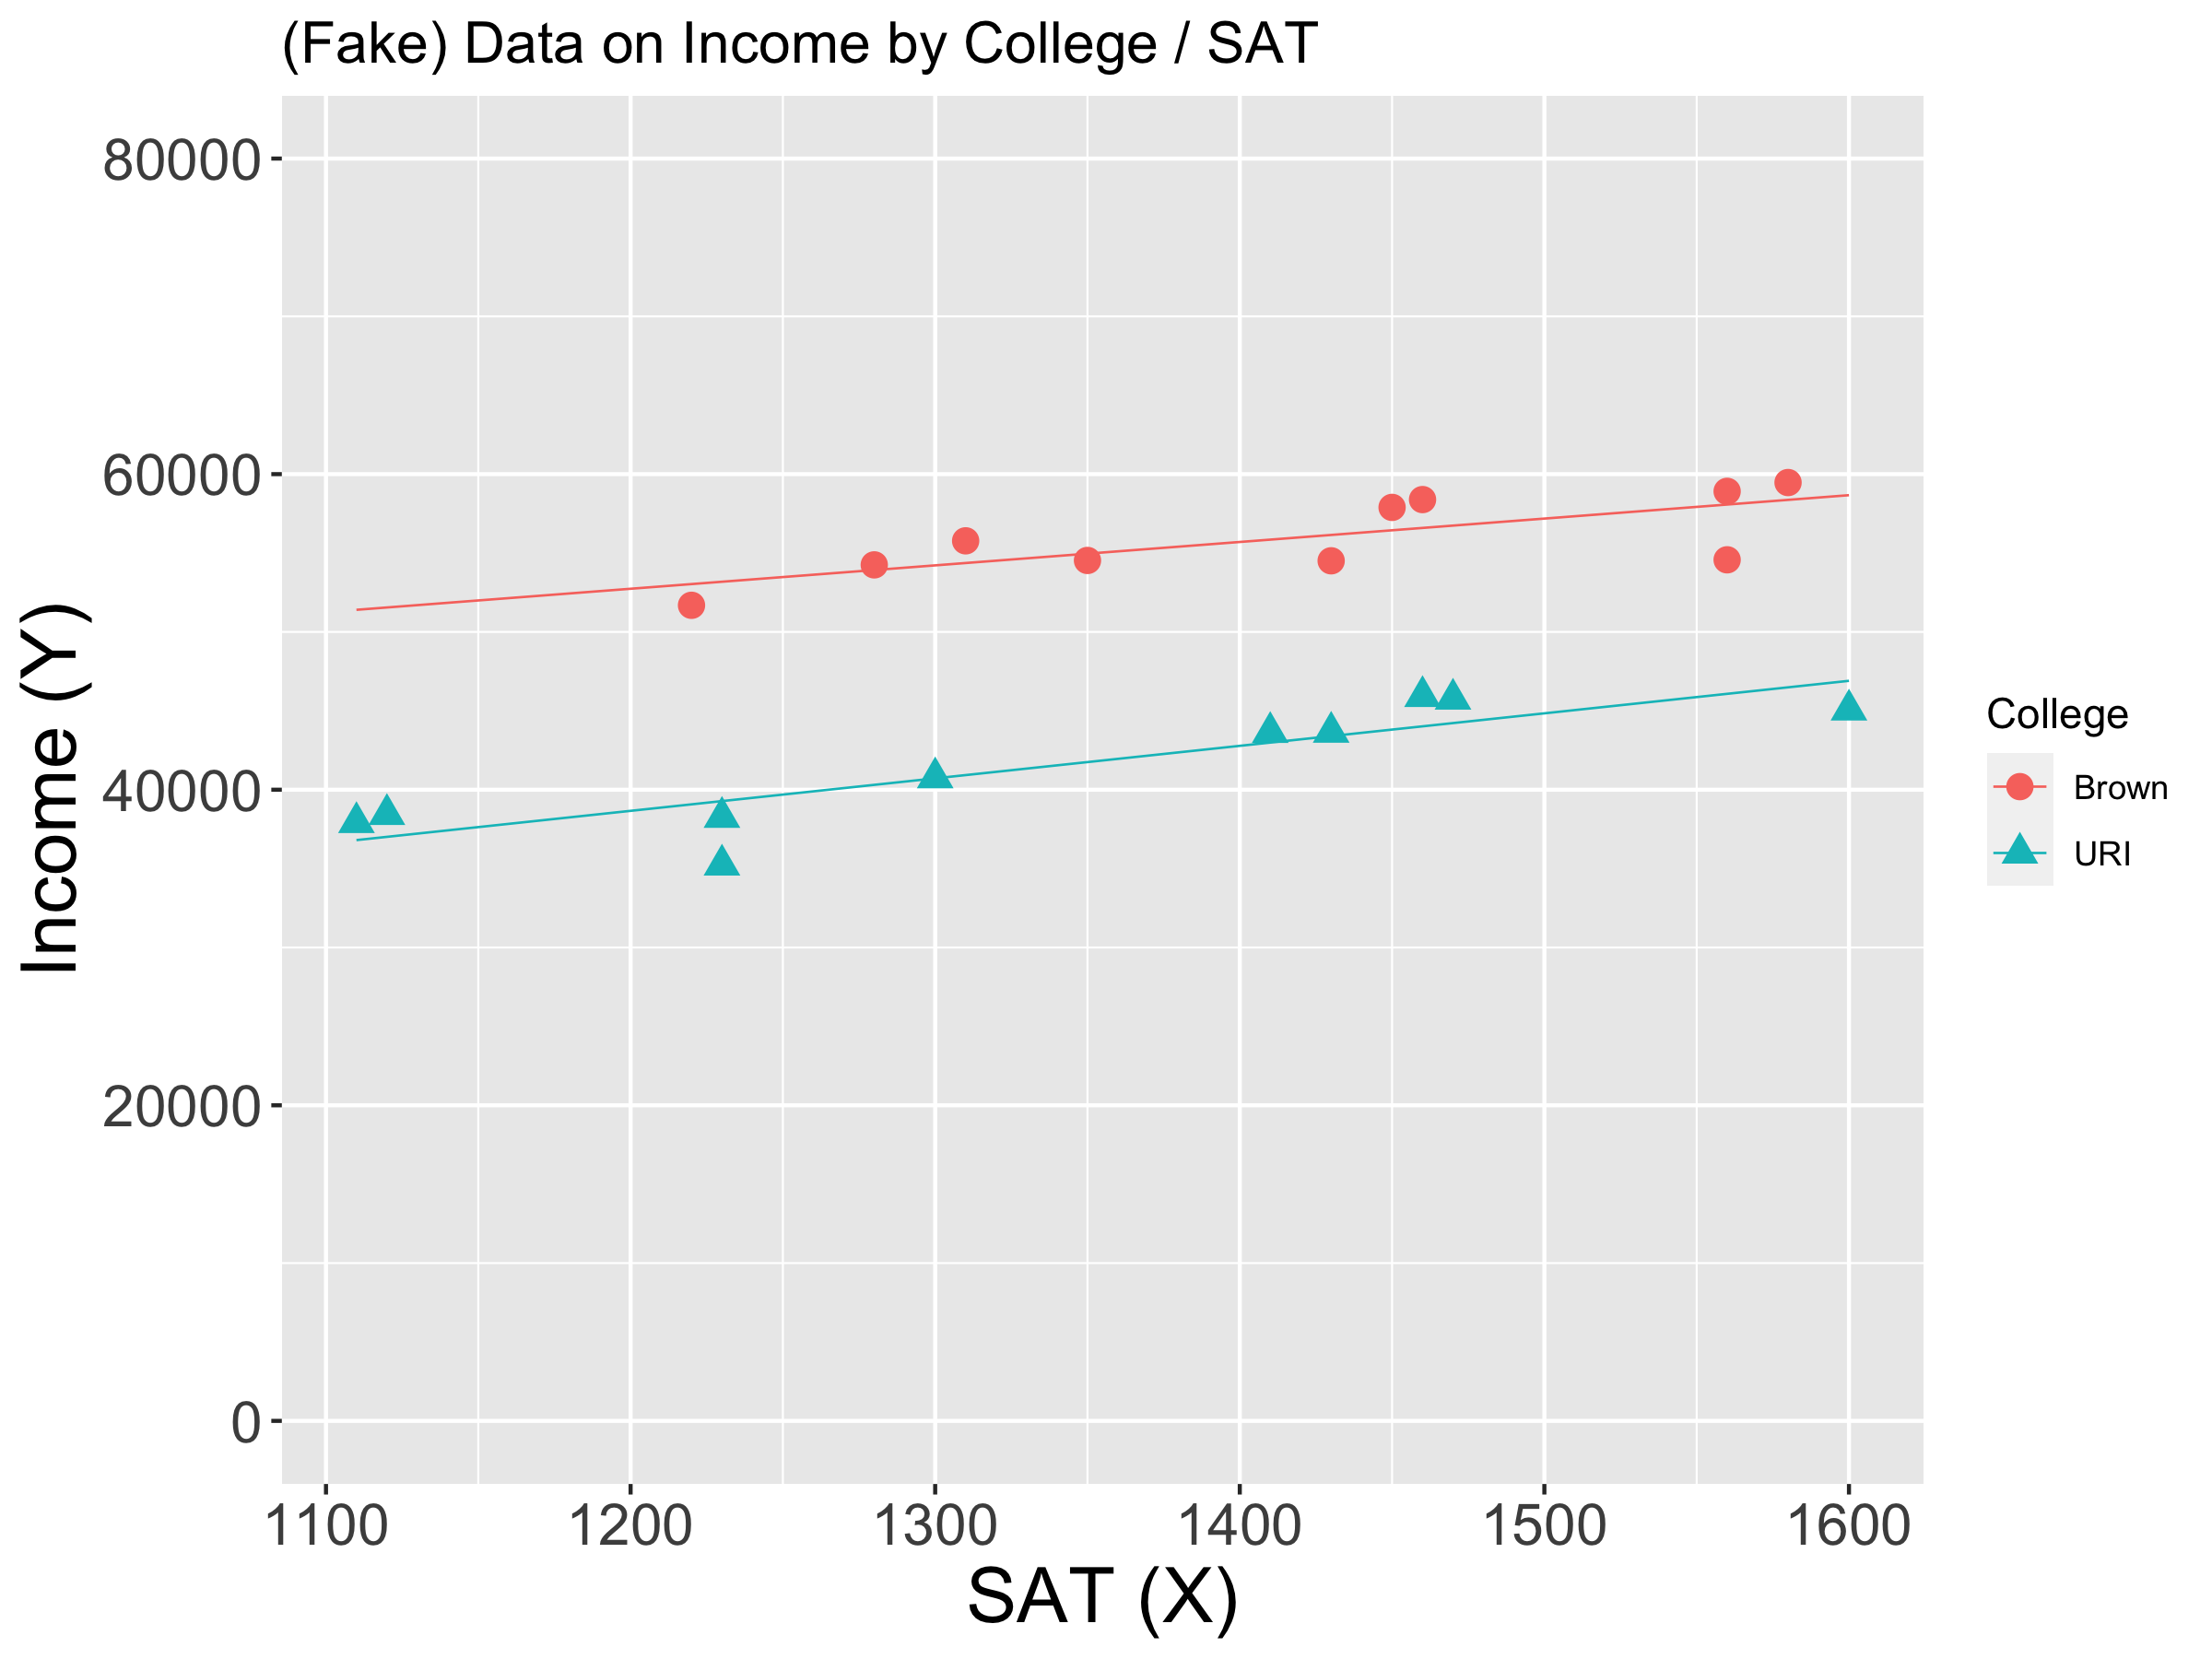
\includegraphics[width = 0.8 \linewidth]{fake-sat-with-trend.png}}
\only<9>{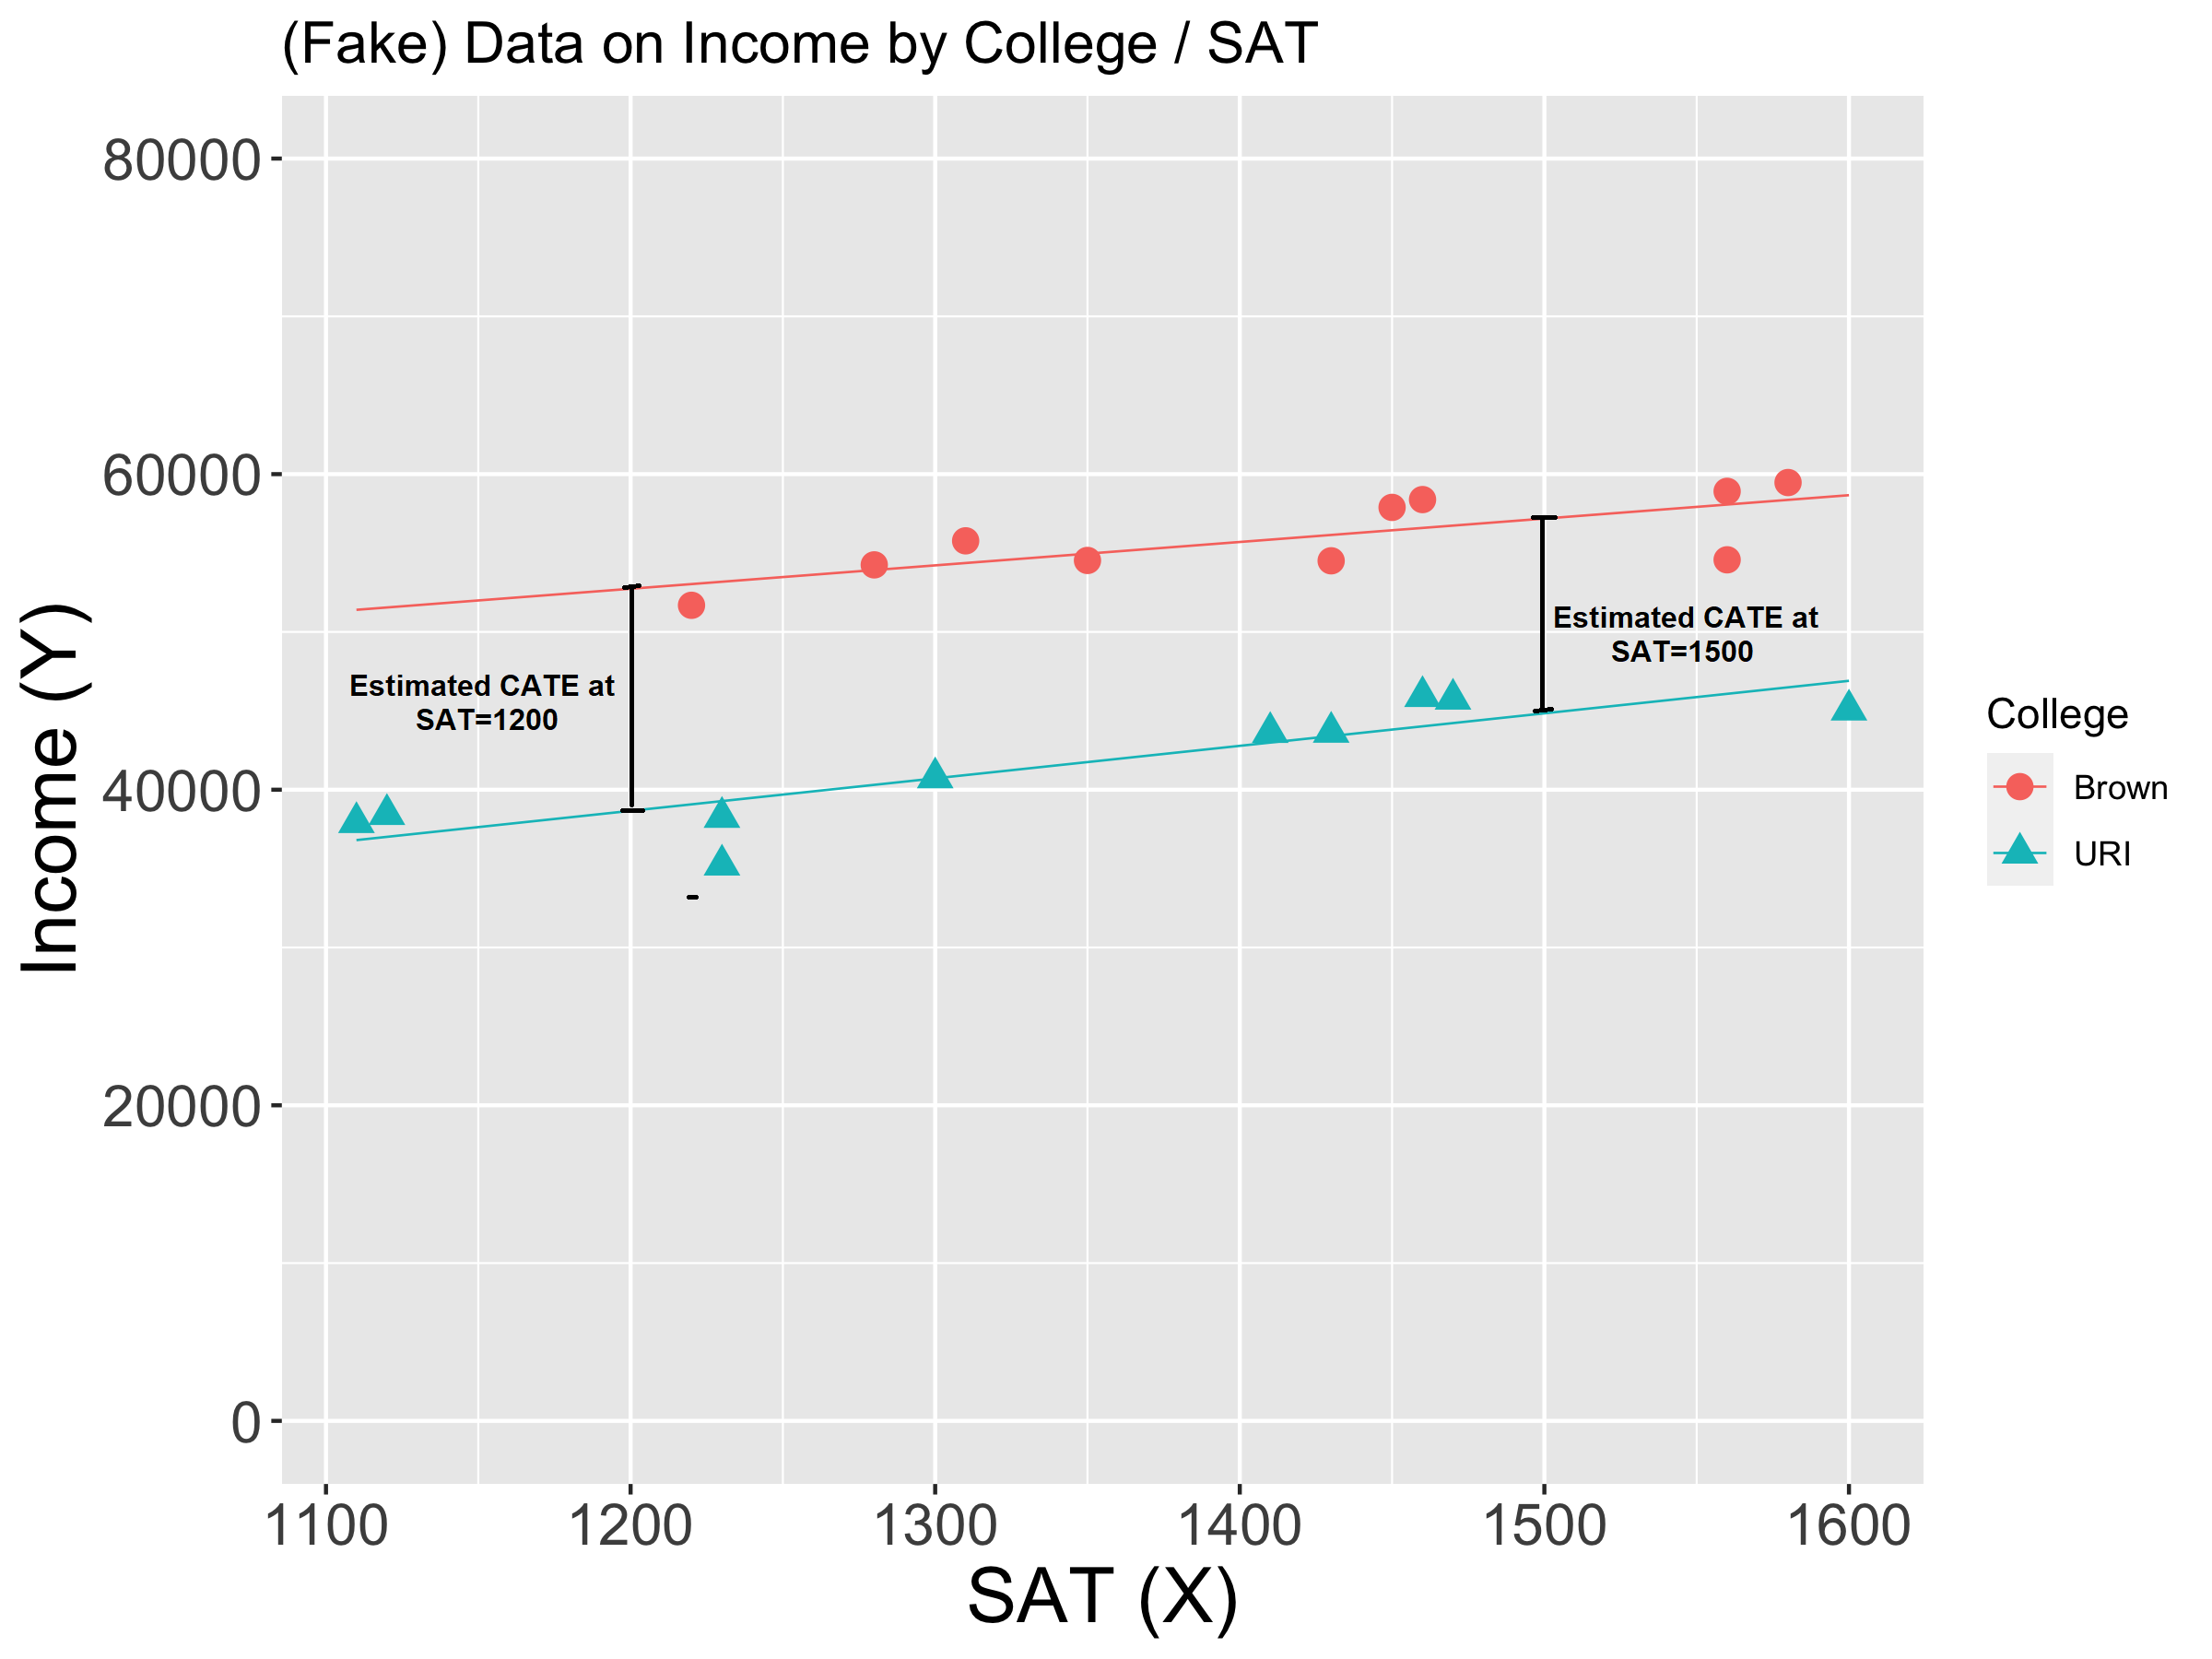
\includegraphics[width = 0.8 \linewidth]{fake-sat-with-trend-annotated2.png}}

\begin{wideitemizeshort}
\only<1> {\item
Suppose this is our data }

\only<2>{
	\item
	We might be willing to assume that college attendance is as-good-as-random conditional on SAT score
}

\only<3>{
\item	
Say we're interested in the CATE at $X=1350$. Theory tells us to compare average income for Brown/URI SAT scores with $X=1350$. 
}

\only<4-5>{
\item
We could estimate the average at Brown using our 1 student with $X=1350$. But that estimate is very noisy, \& we can't apply the CLT
}
\smallskip

\only<5>{
\item
Moreover, we don't have any URI students with $X=1350$!
}

\only<6-8>{
\item
Clearly, we need to extrapolate from students with other SAT scores.

\pause\smallskip
\item<7-8>
What would you do if you were eyeballing it?

\item<8>\smallskip
Probably draw a line through the points to estimate the CEFs!
}

\item<9>
With these CEF estimates in hand, we can estimate $CATE(x)$ at any $x$
\end{wideitemizeshort}
\end{frame}

\begin{frame}{Outline}

1. Population Regression
\vspace{0.8cm}

2. Sample Regressions (OLS)
\vspace{0.8cm}

3. Putting Regression into Practice

\end{frame}

\begin{frame}{Introduction to Regression}
\begin{wideitemize}

\item
The idea of \textbf{regression} is to formalize the process of estimating the conditional expectation function (CEF) by extrapolating across units using a particular functional form (e.g. linear, quadratic, etc.)

\pause
\item
There are a few outstanding questions that we need to answer:

\pause
\item
How do we approximate the CEF in the sample that we have? (I.e. how to draw the lines through the data!)

\pause
\item
How can we construct confidence intervals / do hypothesis tests for the estimates of the CEF? 

\pause
\item
What happens if the real CEF doesn't take the form we've used for estimation (e.g. isn't linear)?

\pause
\item
We'll try to answer all of these questions over the next several lectures!

\end{wideitemize}	
\end{frame}	


\begin{frame}{Roadmap}
\vspace{0.2cm}
\begin{wideitemize}
\item \textbf{What we know how to do:} Estimate and test hypotheses about population means using sample means
\item \textbf{What we want to do:} Estimate approximations to the CEF and test hypotheses about them 
\end{wideitemize}
\pause
\bigskip
How can we use what know to do what we want? 
\pause
\begin{wideitemize}
	\item 1) Assume the CEF takes a particular form, e.g. linear:
	$$E[Y_i | X_i = x] = \alpha + x \beta$$
	
	\pause
	\item 2) Show that under this assumption, $\alpha$ and $\beta$ can be represented as functions of population means.
	
	\pause
	\item
	3) Use our tools for estimating population means using sample means to estimate $\alpha,\beta$ and test hypotheses about them
	
	\pause
	\item
	4) Argue that even if our assumption about the form of the CEF is wrong, the parameters $\alpha,\beta$ may provide a ``good'' approximation.
\end{wideitemize}

\end{frame}


\begin{frame}{The ``Least Squares'' Problem}

\begin{wideitemize}

\item
Suppose $X_i$ is scalar and the CEF is linear (we'll relax both later):
$$E[Y_i | X_i = x] = \alpha + x \beta$$

\pause
\item
A useful fact which we will exploit is that when this is true $(\alpha,\beta)$ solve the ``least squares'' problem:

$$(\alpha,\beta)=\arg\min_{a,b} E[ (Y_i - (a + b X_i))^2  ] $$


\pause
\item
Where does this come from?!


\end{wideitemize}
	
\end{frame}

\begin{frame}{Starting with a Simpler Problem}
\begin{wideitemize}
	\item
	To show that $(\alpha,\beta)$ solve a ``least-squares'' problem, let's first consider a simpler, related problem:
	
	\pause
	\item
	Suppose that we want to find a constant $u$ to minimize 
	$$\min_u E[ (Y_i - u)^2 ]$$
	
	\pause
	\item
	What constant $u$ should we choose? \pause The population mean $\mu=E[Y_i]$!
	
	\pause
	\item
	Proof: \\
	
	The derivative of $E[ (Y_i - u)^2 ]$ with respect to $u$ is $E[ 2(Y_i - u) ]$.  \\ \pause
	
	
	Setting the derivative to 0, we obtain
	$$E[ 2(Y_i - \mu) ] = 0 \Rightarrow 2 E[Y_i] = 2 u \Rightarrow u = E[Y_i].$$
	
\end{wideitemize}	
\end{frame}

\begin{frame}{Now A Slightly Harder Problem}
\vspace{0.2cm}
\begin{wideitemize}

	\item
	Now suppose we want to choose the function $u(x)$ to minimize
	$$\min_{u(\cdot)} E[ (Y_i - u(X_i))^2  ]$$
	
	\pause
	\item
	What function $u(x)$ should we choose? \pause The conditional expectation $u(x) = E[Y|X= x]$. 
	
	\pause
	\item
	Proof: \\
	By the law of iterated expectations,
	$$E[ (Y_i - u(X_i))^2  ] = E[  E[  (Y_i - u(X_i)) ^2| X_i  ]   ] .$$
	
	\pause
	Thus, for each value of $x$, we want to choose $u(x)$ to minimize
	$$E[ (Y_i - u(x))^2 | X_i = x ].$$ 
	
	\pause However, our argument on the previous slide implies that the solution is $u(x) = E[Y_i | X_i = x]$. 
\end{wideitemize}
\end{frame}

\begin{frame}{Looping Back...}
	
\begin{wideitemize}

\item
We've shown that the function $u(x) = E[Y_i | X_i = x]$ solves
$$\min_{u(\cdot)} E[ (Y_i - u(X_i))^2  ]$$

\pause
\item
Thus, if $E[Y_i | X_i = x] = \alpha + \beta x$, then $u(x) = \alpha + \beta x$ minimizes  
$$\min_{u(\cdot)} E[ (Y_i - u(X_i))^2  ]$$

\pause
\item
The minimization above was over \textit{all} functions $u(\cdot)$, including linear ones of the form $a + b x$. Hence, 

$$ E[ (Y_i -  (\alpha + \beta X_i)  )^2  ] \leq  E[ (Y_i -  (a + b X_i)  )^2  ]  \text{ for all } a ,b. $$

\pause
\item
This implies that $(\alpha,\beta)$ solve

$$\min_{a,b}E[ (Y_i -  (a+ b X_i)  )^2  ] ,$$

\noindent as we wanted to show
\end{wideitemize}	
\end{frame}


\begin{frame}{Why This is Useful}
\begin{wideitemize}

\item
So we've shown that $\alpha,\beta$ are the solutions to 

$$\min_{a,b}E[ (Y_i -  (a+ b X_i)  )^2  ] .$$

\item 
How does this help us? \pause By solving the minimization problem, we can express $\alpha,\beta$ as functions of population expectations. 

\pause
\item
Let's take the derivative w.r.t. $a$ and $b$ and set them to zero at $(\alpha,\beta)$: \pause
\begin{align*}
& E[-2  (Y_i - (\alpha + \beta X_i )) ] = 0 \\ \pause
& E[-2  X_i (Y_i -(\alpha + \beta X_i)) ] = 0
\end{align*}

\pause
\item
We now have 2 equations with 2 unknowns, which we can use to solve for the CEF parameters $(\alpha,\beta)$

\end{wideitemize}
\end{frame}

\begin{frame}{The Least Squares Solution}
\begin{wideitemize}
\item
The solution to the system of equations is as follows:
\begin{align*}
& \beta = \frac{E[ (X_i -E[X_i]) (Y_i - E[Y_i])  ]}{E[ (X_i - E[X_i])^2 ]} = \frac{Cov(X_i, Y_i)}{Var(X_i)} \\ 
& \alpha = E[Y_i] - E[X_i] \beta
\end{align*}

\pause
\item
These are continuous functions of population means!

\pause
\item
We can therefore use the tools from previous lectures to estimate them and test hypotheses about the CEF! 
\end{wideitemize}	
\end{frame}


\begin{frame}{Roadmap}
	\begin{wideitemize}
		\item \textbf{What we know how to do:} Estimate and test hypotheses about population means using sample means
		\item \textbf{What we want to do:} Estimate approximations to the CEF and test hypotheses about them 
	\end{wideitemize}
	\bigskip
	How can we use what know to do what we want? 

	\begin{wideitemize}
		\item 1) Assume the CEF takes a particular form, e.g. linear:
		$$E[Y_i | X_i = x] = \alpha + x \beta \hspace{2cm }\checkmark$$
		
		\item 2) Show that under this assumption, $\alpha$ and $\beta$ can be represented as functions of population means. $\checkmark$
		
		\item
		3) Use our tools for estimating population means using sample means to estimate $\alpha,\beta$ and test hypotheses about them
		
		\item
		4) Argue that even if our assumption about the form of the CEF is wrong, the parameters $\alpha,\beta$ may provide a ``good'' approximation.
	\end{wideitemize}
	
\end{frame}

\begin{frame}{Outline}

\textcolor{red!75!green!50!blue!25!gray}{1. Population Regression}$\checkmark$
\vspace{0.8cm}

2. Sample Regressions (OLS)
\vspace{0.8cm}

\textcolor{red!75!green!50!blue!25!gray}{3. Putting Regression into Practice}

\end{frame}


\begin{frame}{Estimating Regression Coefficients}
	\begin{wideitemize}
	\item
	We showed that  when $E[Y_i\mid X_i=x]=\alpha+\beta x$
\begin{align*}
& \beta = \frac{E[ (X_i -E[X_i]) (Y_i - E[Y_i])  ]}{E[ (X_i - E[X_i])^2 ]} = \frac{Cov(X_i, Y_i)}{Var(X_i)} \\ 
& \alpha = E[Y_i] - E[X_i] \beta
\end{align*}
	
	\item
	How can we estimate $\alpha,\beta$? \pause \\ Replace population means with sample averages!
	\pause
	\begin{align*}
		& \hat\beta = \dfrac{ \frac{1}{N} \sum_{i=1}^{N} (X_i - \bar{X})(Y_i - \bar{Y})  }{ \frac{1}{N} \sum_{i=1}^N (X_i - \bar{X})^2 } =\frac{\widehat{Cov}(X_i,Y_i)}{\widehat{Var}(X_i)}\pause{} \\
		& \hat\alpha = \bar{Y} - \bar{X} \hat{\beta}
	\end{align*}

	
	\pause
	\item
	These $\hat\alpha,\hat\beta$ are called \textit{ordinary least squares} (OLS) coefficients\smallskip
\begin{itemize}
\item They solve the ``sample analog'' problem, $\min_{a,b}\frac{1}{N}\sum_i (Y_i -  (a+ b X_i)  )^2   $
\end{itemize}
	\end{wideitemize}	
\end{frame}


\begin{frame}
	\centering
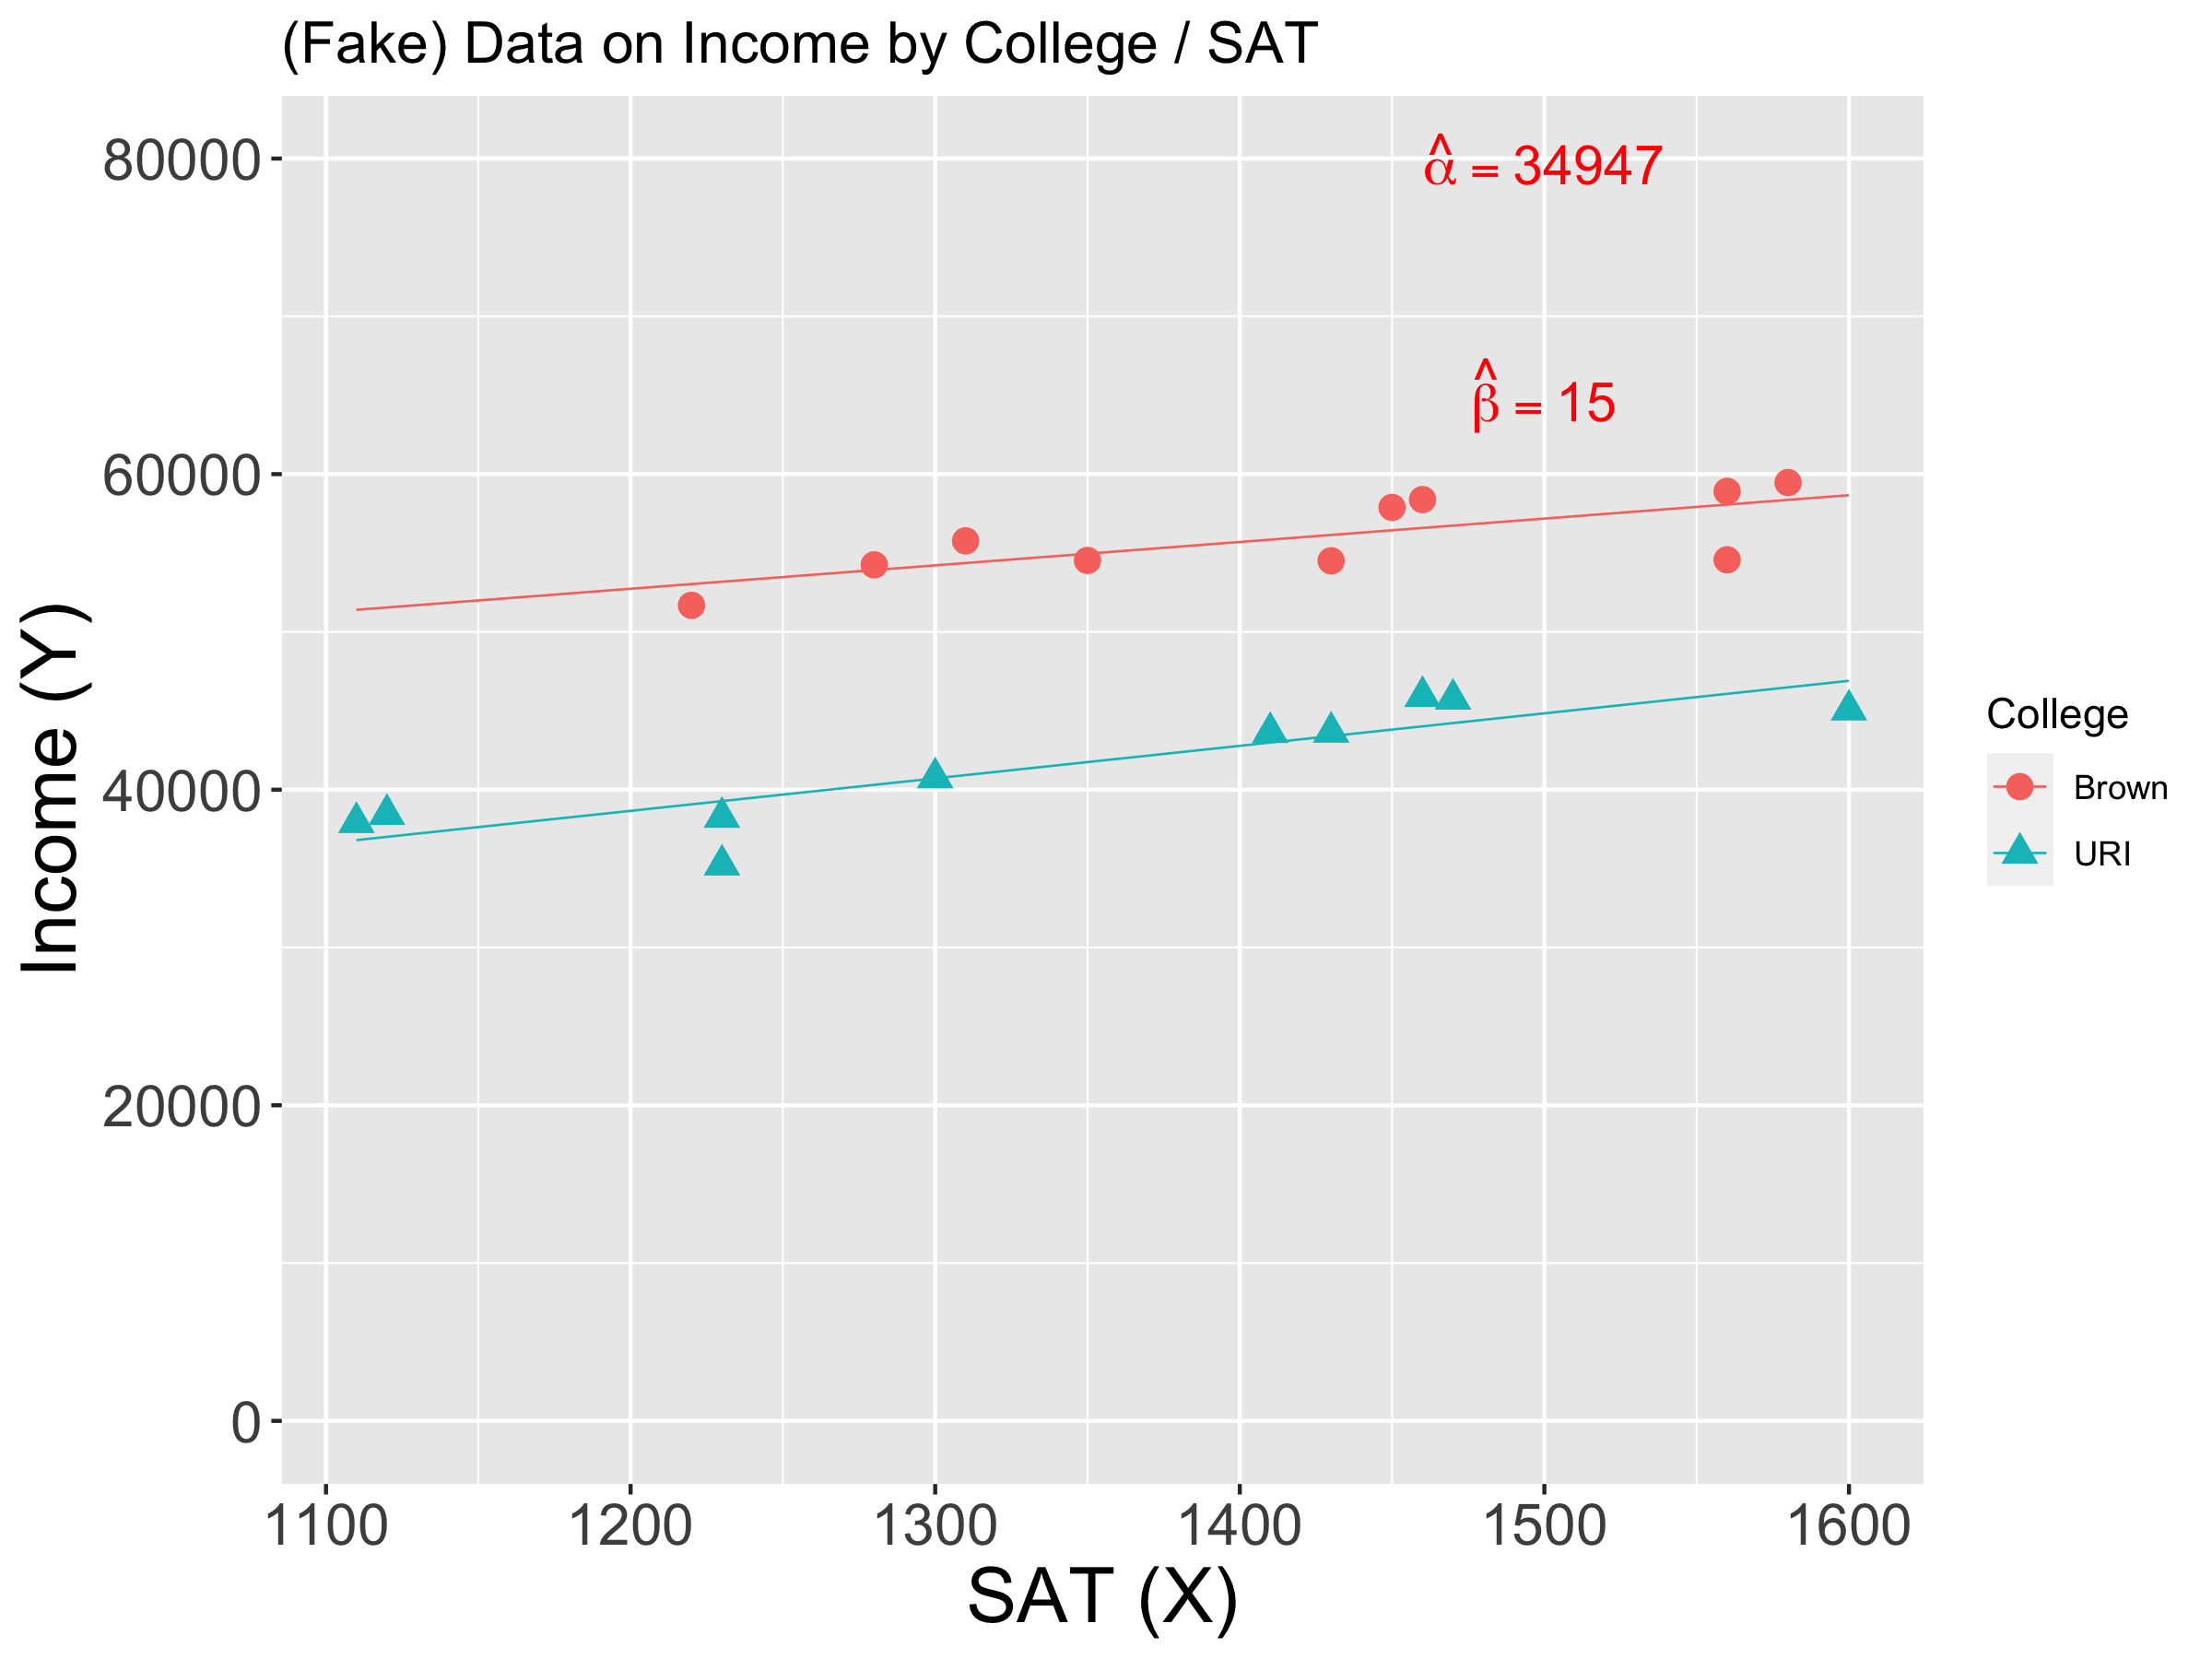
\includegraphics[width = .9\linewidth]{fake-sat-with-trend-brown-betas.png}
\end{frame}

\begin{frame}
	\centering
	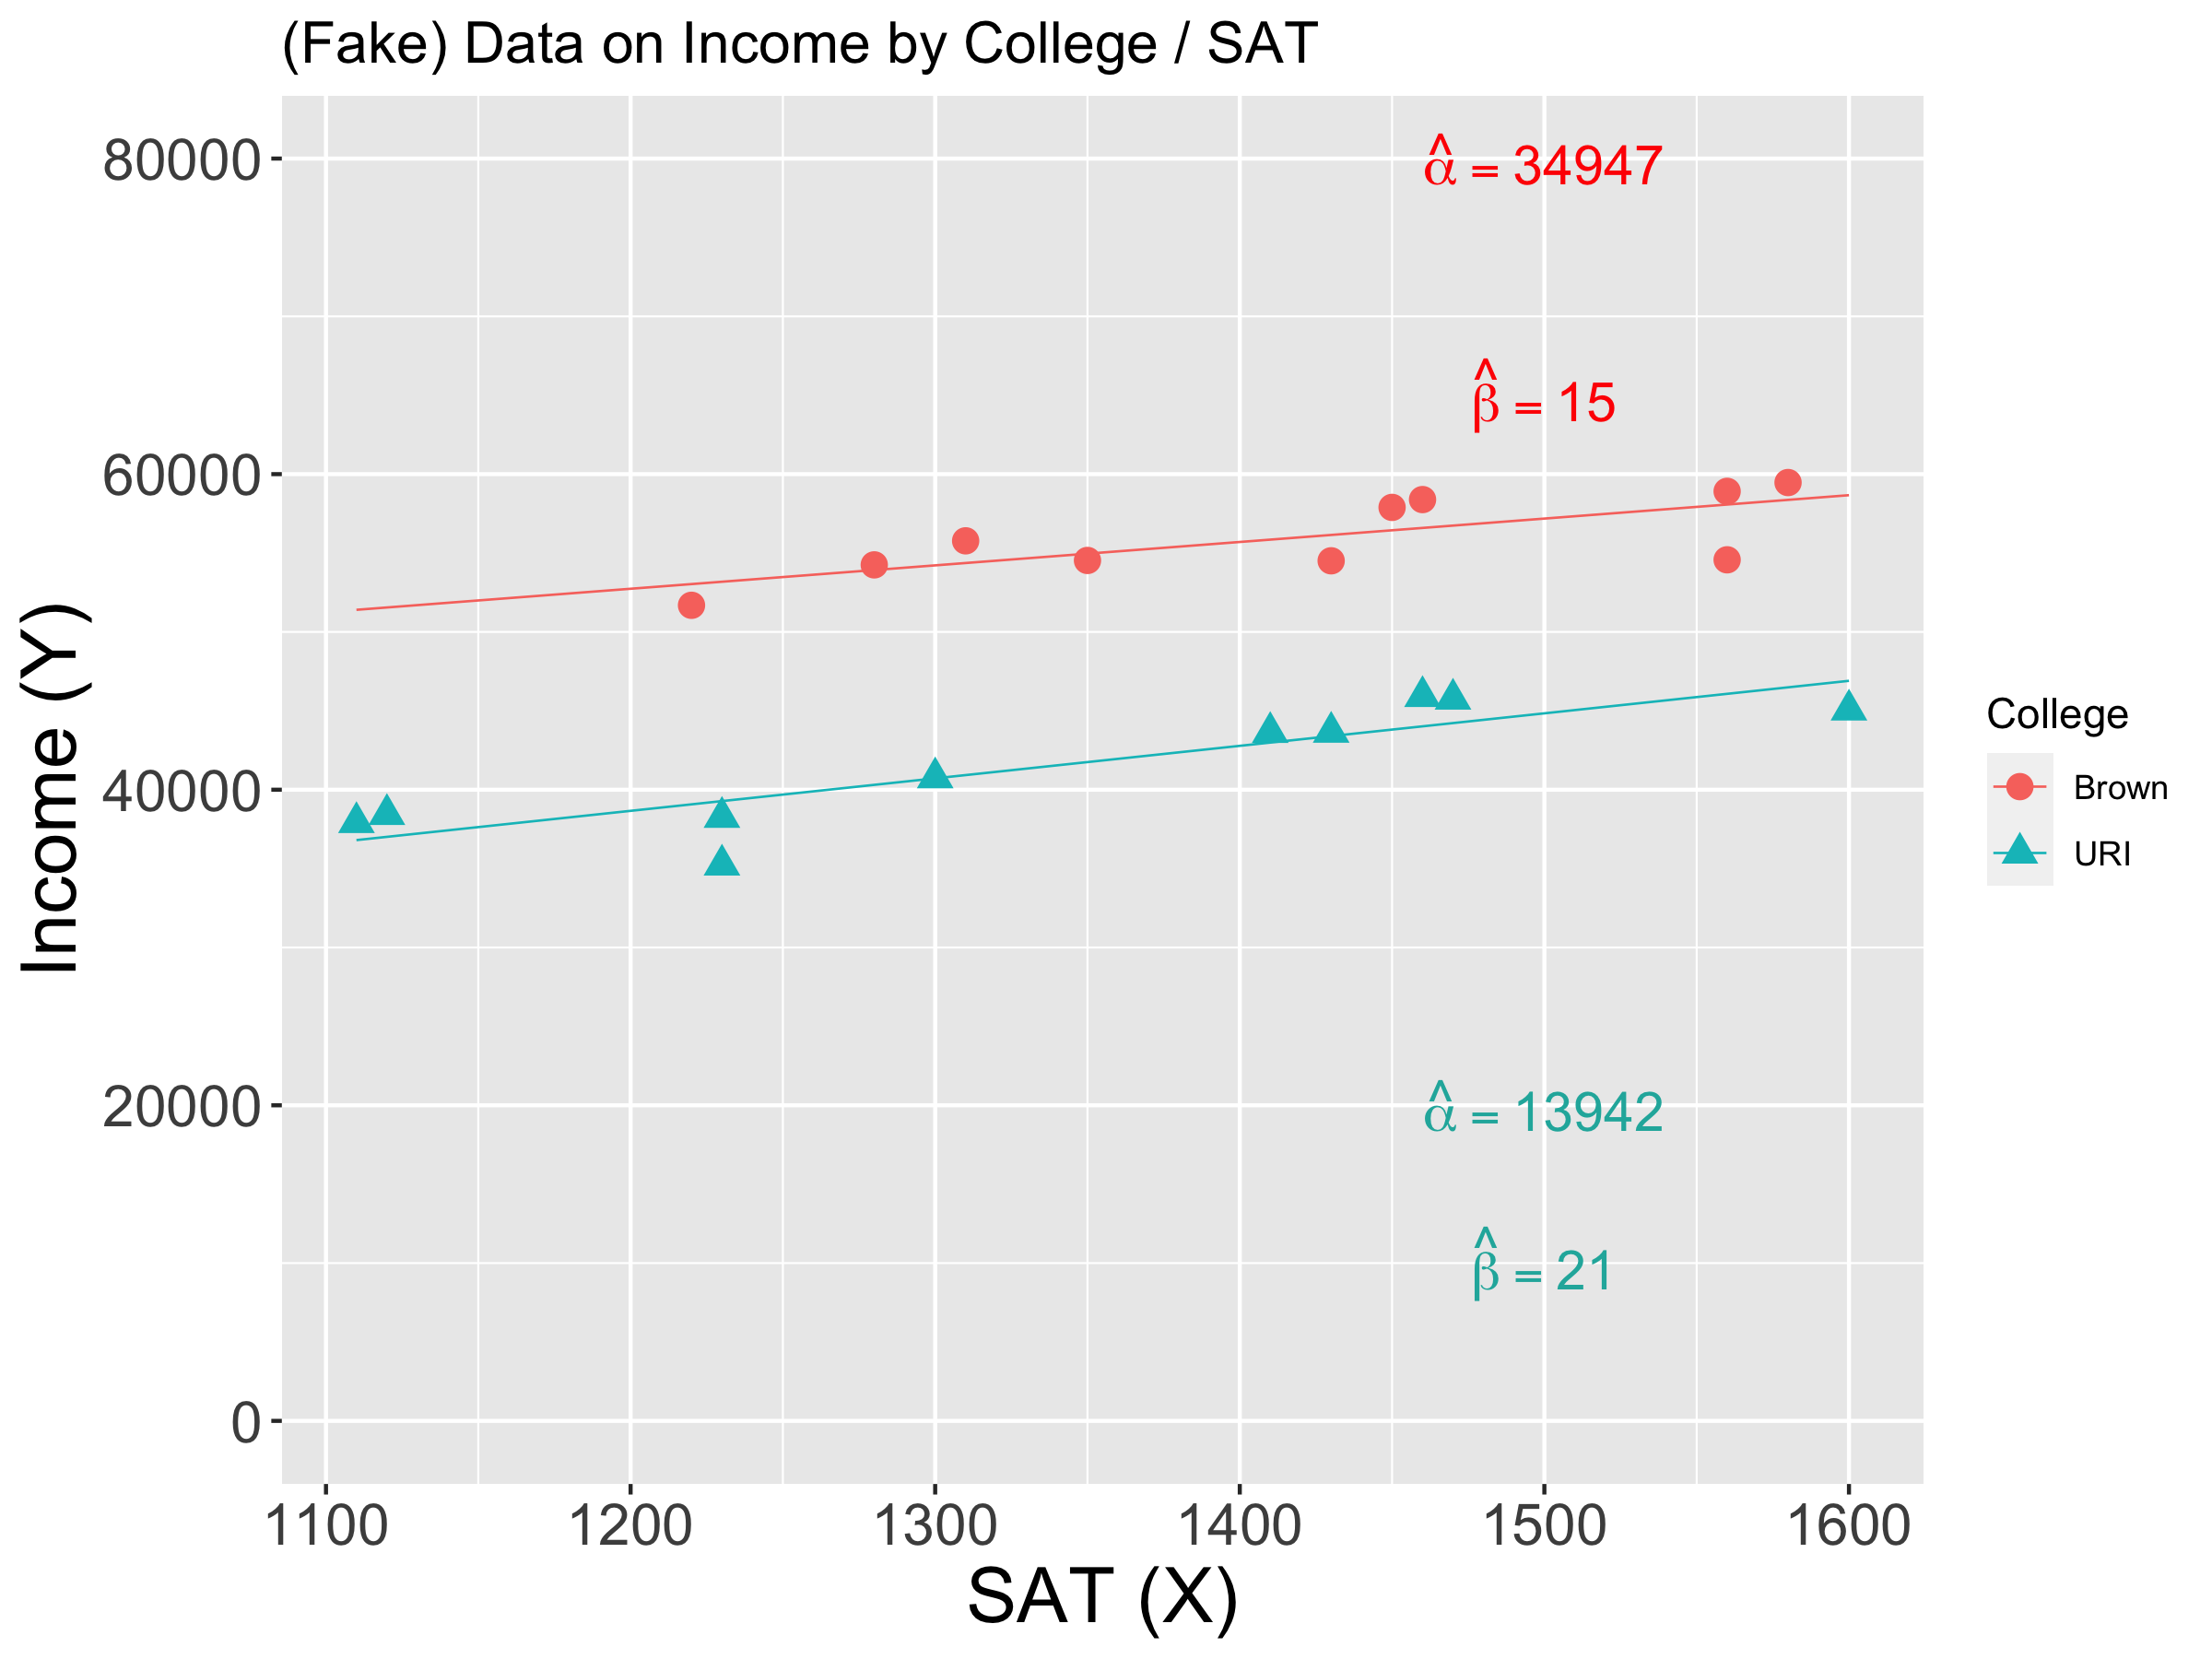
\includegraphics[width =.9\linewidth]{fake-sat-with-trend-both-betas.png}
	
	\pause
	\begin{wideitemize}
		\item
		What is the estimated value of $E[Y_i | D_i = 1, X_i = 1350]$? \pause $\hat\alpha + \hat\beta \cdot 1350 = 34947 + 15 \cdot 1350 = 55197$. 
	\end{wideitemize}
\end{frame}


%\begin{frame}{Estimating $CATE(x)$}
%\begin{wideitemize}
%\item
%Remember that under conditional unconfoundedness: 
%$$CATE(x) = E[ Y_i |D_i = 1, X_i =x ] - E[Y_i |D_i =0, X_i  = x]$$
%
%\item
%Under our assumption that 
%\end{wideitemize}	
%\end{frame}

\begin{frame}{Consistency of OLS}
\begin{wideitemize}
\item
We can now use our results for (functions of) sample averages to show that $\hat\beta$ is consistent for $\beta$, i.e. $\hat\beta \rightarrow_p \beta$.

\pause
\item
We have that
\begin{align*}
 \hat\beta &=\left( \frac{1}{N} \sum_{i=1}^N (X_i - \bar{X})^2 \right)^{-1}   \frac{1}{N} \sum_{i=1}^{N} (X_i - \bar{X})(Y_i - \bar{Y}) \pause{}  \\
 &= \left( \frac{1}{N} \sum_{i=1}^N X_i^2 - \bar{X}^2 \right)^{-1}   \left( \frac{1}{N} \sum_{i=1}^{N} X_i Y_i - \bar{X} \bar{Y} \right) \pause{} \\
 & \rightarrow_p \left( E[X_i^2] - E[X_i]^2 \right)^{-1}   \left( E[X_i Y_i] - E[X_i] E[Y_i] \right) \pause{} \\
 &= Var(X_i)^{-1} Cov(X_i, Y_i) \pause{} = \beta
\end{align*}


\pause
\item
Analogously, we can show that $\hat\alpha \rightarrow_p \alpha$.
\end{wideitemize}		
\end{frame}


\begin{frame}{Asymptotic Distribution for OLS}
	\begin{wideitemize}
	\item
	Our OLS estimates $\hat\alpha, \hat\beta$ are continuous functions of sample means.
	
	\pause
	\item
	We can therefore use the Central Limit Theorem and Continuous Mapping Theorem to show that they are asymptotically normally distributed
	
	\pause
	\item
	In particular, we will show that
	
		$$\sqrt{N}(\hat\beta - \beta) \rightarrow_d N(0, \sigma^2),$$
	
	\noindent where
	
	$$\sigma^2 = \dfrac{  Var((X_i - E[X_i])\epsilon_i) }{ Var(X_i)^2  }$$ 
	
	
	\pause
	\item
	This is useful because we can then form CIs for $\beta$ of the form $\hat\beta 	\pm 1.96 \hat\sigma / \sqrt{N}$, where $\hat\sigma$ is our estimate of $\sigma$. 
	
	\end{wideitemize}	
\end{frame}

\begin{frame}{Deriving the Asymptotic Distribution for OLS}
\begin{wideitemize}

\item
Define the \textbf{regression residual} $\epsilon_i = Y_i - (\alpha+X_i \beta)$, implying
\begin{equation*}
Y_i = \alpha + X_i \beta + \epsilon_i	
\end{equation*}

\pause
\item
The first-order conditions we derived for $(\alpha,\beta)$ imply this residual is mean-zero and \textbf{orthogonal} to the \textbf{regressor}: $E[\epsilon_i] = E[X_i \epsilon_i] =0$

\pause
\item
Taking means, $\bar{Y} = \alpha + \bar{X} \beta + \bar{\epsilon}$. \pause So $Y_i - \bar{Y} = (X_i - \bar{X})\beta + (\epsilon_i-\bar\epsilon)$

\end{wideitemize}

\end{frame}

\begin{frame}{Asymptotic Distribution for OLS (cont.)}
	\begin{wideitemize}
		
		\item
		We just derived that $Y_i - \bar{Y} = (X_i - \bar{X})\beta + (\epsilon_i-\bar\epsilon)$. 
		
		\item
		Thus,
		\begin{align*}
			\hat\beta &=\left( \frac{1}{N} \sum_{i=1}^N (X_i - \bar{X})^2 \right)^{-1}   \frac{1}{N} \sum_{i=1}^{N} (X_i - \bar{X})(Y_i - \bar{Y})   \\
			&=\pause{} \left( \frac{1}{N} \sum_{i=1}^N (X_i - \bar{X})^2 \right)^{-1}   \frac{1}{N} \sum_{i=1}^{N} (X_i - \bar{X})((X_i - \bar{X})\beta + (\epsilon_i-\bar\epsilon) ) \pause{} \\
			& =\beta + \left( \frac{1}{N} \sum_{i=1}^N (X_i - \bar{X})^2 \right)^{-1}   \frac{1}{N} \sum_{i=1}^{N} (X_i - \bar{X}) (\epsilon_i - \bar\epsilon)
		\end{align*}
\end{wideitemize}	
\end{frame}

\begin{frame}{Asymptotic Distribution for OLS (cont.)}
\begin{wideitemize}
	\item	Hence,
	\begin{align*}
		\sqrt{N}(\hat\beta - \beta) &= \left( \frac{1}{N} \sum_{i=1}^N (X_i - \bar{X})^2 \right)^{-1}  \sqrt{N} \frac{1}{N} \sum_{i=1}^N (X_i - \bar{X})(\epsilon_i - \bar{\epsilon}) \pause{} \\
		&= \left( \frac{1}{N} \sum_{i=1}^N (X_i - \bar{X})^2 \right)^{-1} \sqrt{N}\frac{1}{N} \sum_{i=1}^N (X_i - E[X_i])\epsilon_i \\
		&-\left( \frac{1}{N} \sum_{i=1}^N (X_i - \bar{X})^2 \right)^{-1}  \left( \bar{\epsilon} \sqrt{N} (\bar{X} - E[X_i]) \right)
	\end{align*}

	\item
	By LLN and CMT, $\left( \frac{1}{N} \sum_{i=1}^N (X_i - \bar{X})^2 \right)^{-1} \rightarrow_p Var(X_i)^{-1}$
	
	\pause
	\item
	By CLT, $\sqrt{N}\frac{1}{N} \sum_{i=1}^N (X_i - E[X_i])\epsilon_i \rightarrow_d \mathrm{N}(0, Var((X_i - E[X_i])\epsilon_i)).$
	
	\pause
	\item
	By LLN, CLT, and Slutsky,  $\bar{\epsilon} \sqrt{N} (\bar{X} - E[X_i]) \rightarrow_d 0 \times \mathrm{N}(0, Var(X_i))  = 0$
	
\end{wideitemize}

\end{frame}

\begin{frame}{Finishing the Asymptotics (!)}
	
	\begin{wideitemize}
	\item
	Putting all the pieces together, we see that
	
	$$\sqrt{N}(\hat\beta - \beta) \rightarrow_d N(0, \sigma^2),$$
	
	\noindent where
	
	$$\sigma^2 = \dfrac{  Var((X_i - E[X_i])\epsilon_i) }{ Var(X_i)^2  }$$ 
	
	\item
	As before, we can estimate the variance $\sigma^2$ using sample averages,
	
	$$\hat\sigma^2 = \dfrac{  \frac{1}{N} \sum_i ((X_i - \bar{X})\hat\epsilon_i )^2}{ \left(\frac{1}{N} \sum_i (X_i - \bar{X})^2\right)^2  }, \text{ where } \hat\epsilon_i = Y_i - (\hat\alpha + X_i \hat\beta)$$ 
	
	
	\item
	\pause
	Can do similar steps to show $\hat\alpha$ is asymptotically normally distributed as well. (We'll show formulas later!)
\end{wideitemize}	
\end{frame}
		
		
\begin{frame}
	\centering
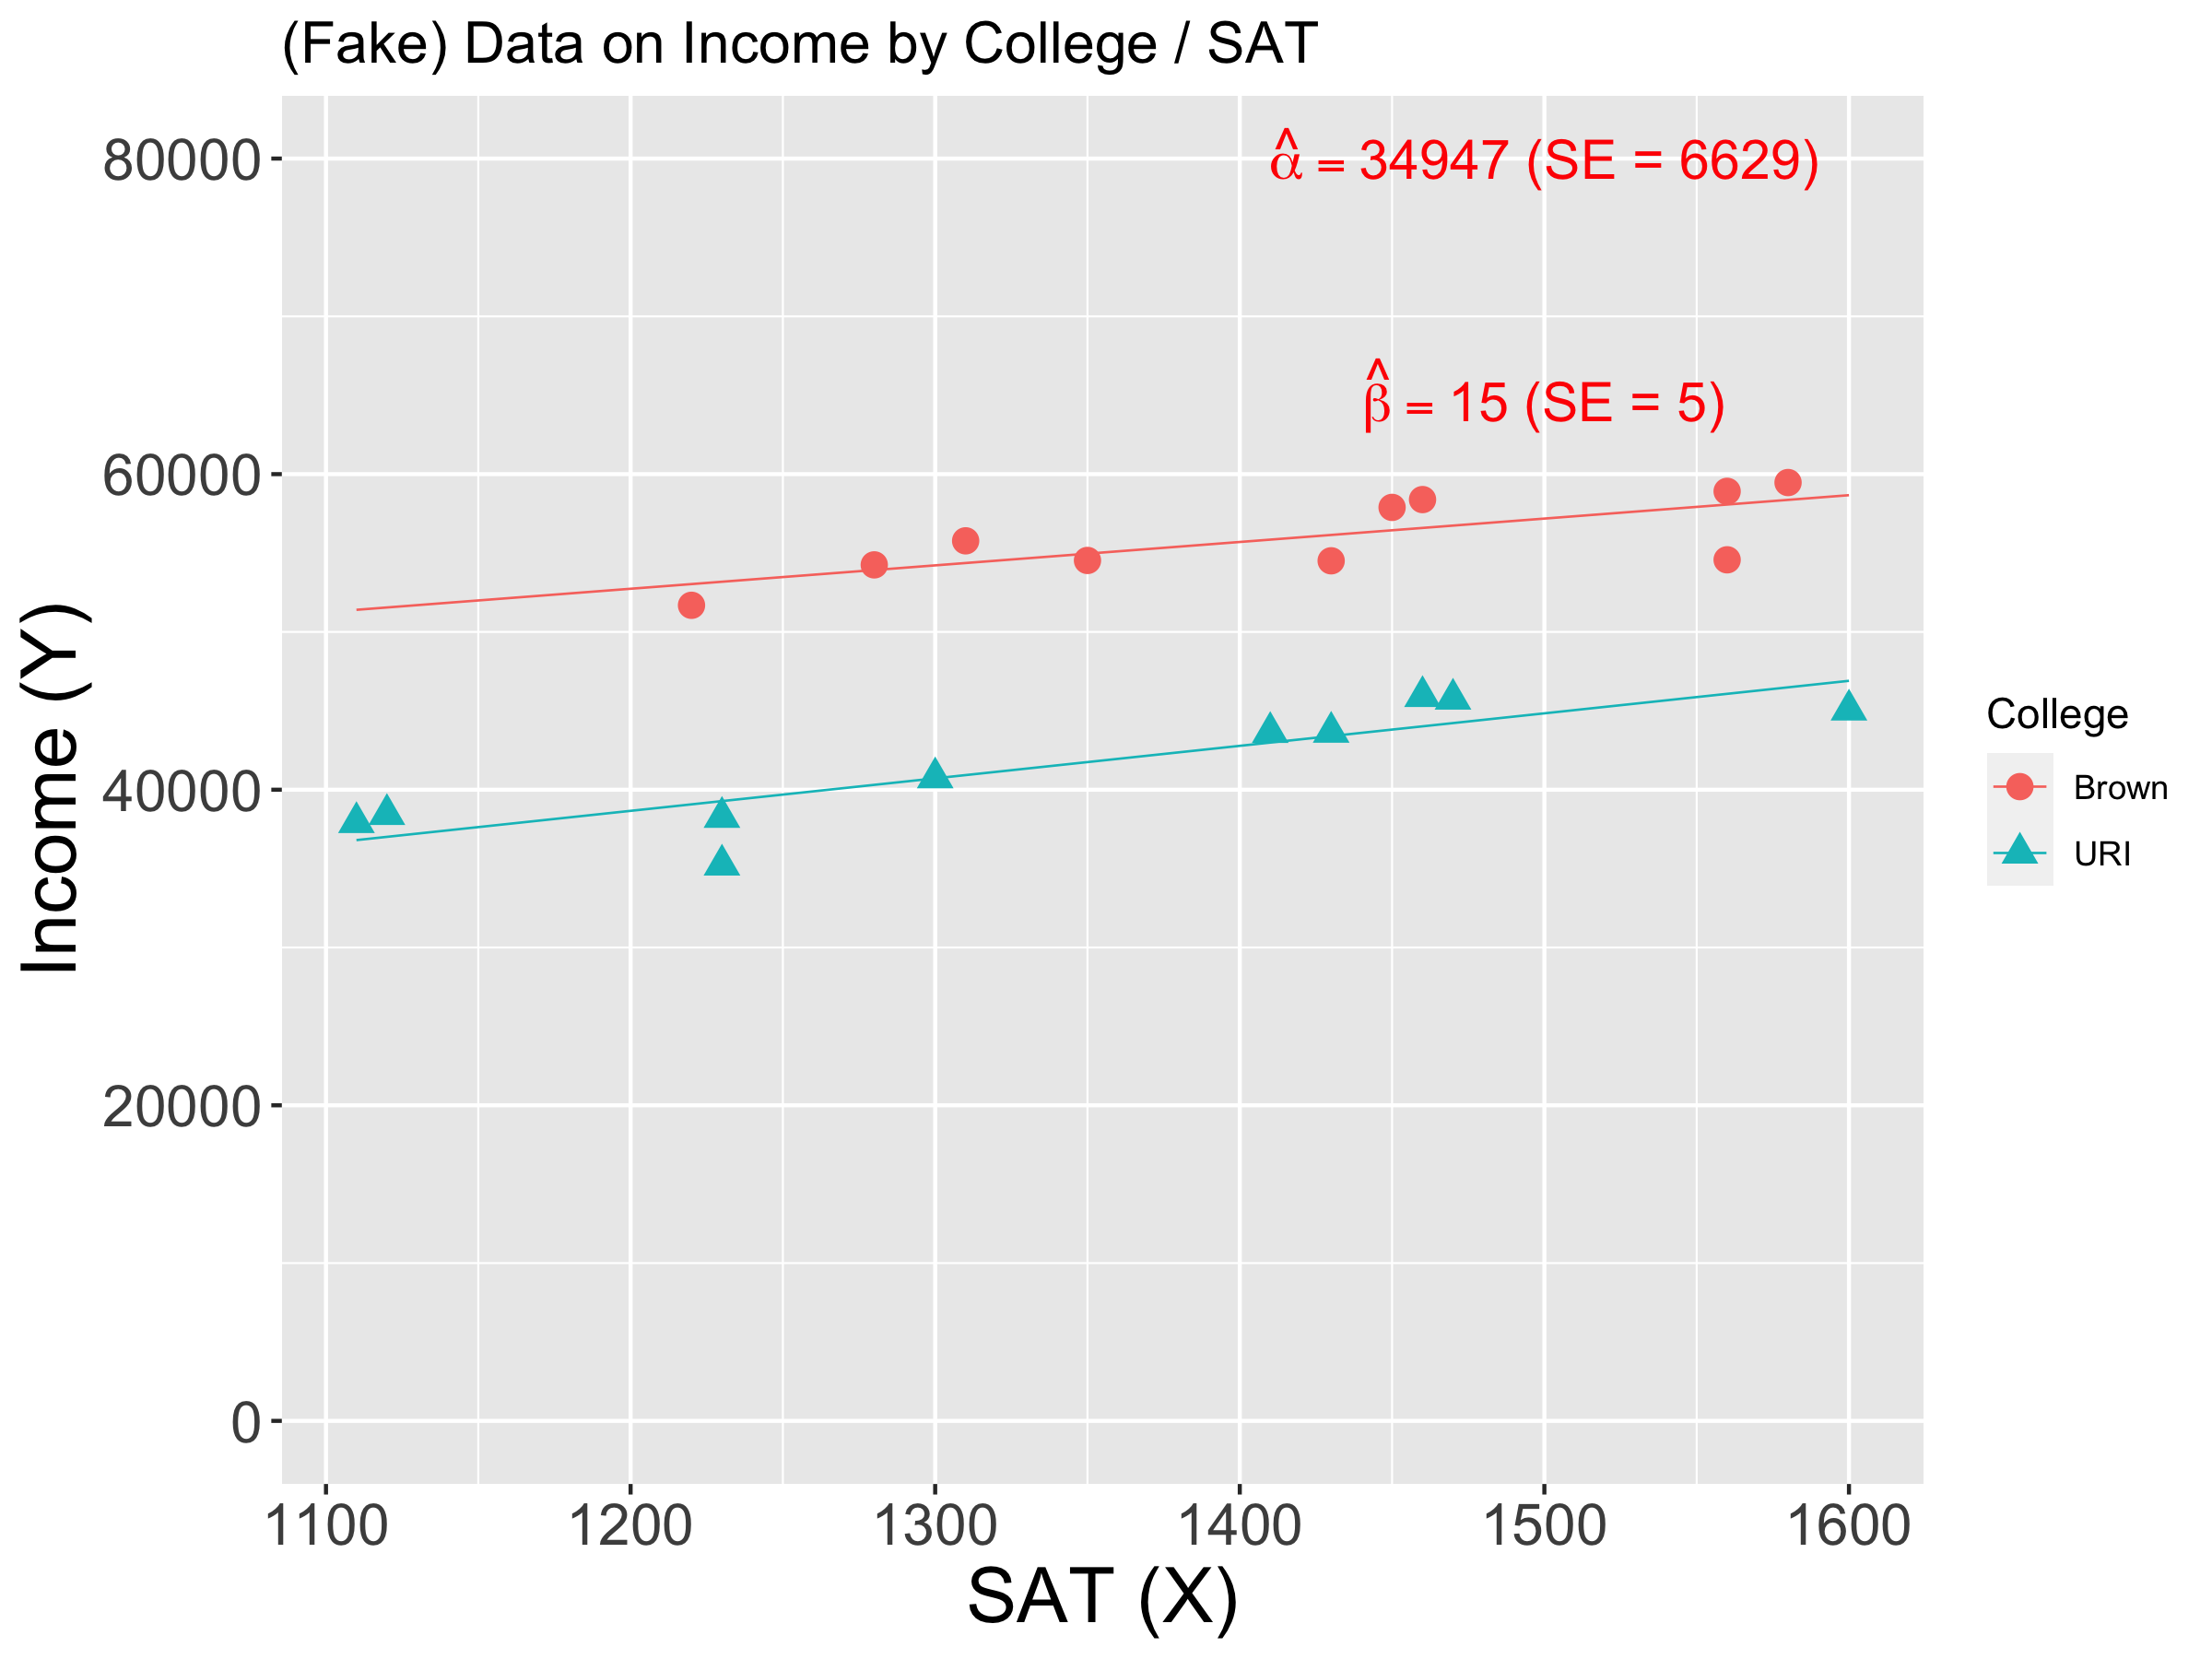
\includegraphics[width = 0.8\linewidth]{fake-sat-with-trend-brown-betas-plus-ses.png}

\pause

\begin{wideitemize}
	\item
	A CI for $\beta$ is $\hat\beta \pm 1.96 \times SE \pause{} \approx [5,25]$
\end{wideitemize}
\end{frame}		
		
\begin{frame}{Aside on notation/terminology}
\begin{wideitemize}
	\item
	Oftentimes people will say: consider the (population) regression
	\begin{equation}
		Y_i = \alpha + \beta D_i + \epsilon_i \label{eqn: pop regression}
	\end{equation}	

	\item
	What they mean is: ``define $(\alpha,\beta) = \arg\min_{a,b} E[ (Y_i - (a + b X_i))^2 ]$''
	
	\item
	$(\alpha,\beta)$ are referred to as the ``population regression coefficients''
	
	\pause
	\item
	Likewise, people will say ``We estimate equation (\ref{eqn: pop regression}) by OLS'' to mean that they compute the sample analogs to $\alpha,\beta$ via OLS, i.e. $\hat\alpha, \hat\beta$.  
\end{wideitemize}
	
\end{frame}		
		
\begin{frame}{Outline}

\textcolor{red!75!green!50!blue!25!gray}{1. Population Regression}$\checkmark$
\vspace{0.8cm}

\textcolor{red!75!green!50!blue!25!gray}{2. Sample Regressions (OLS)}$\checkmark$
\vspace{0.8cm}

3. Putting Regression into Practice

\end{frame}
		
\begin{frame}{Using Regressions to Analyze RCTs}
	\begin{wideitemize}
		\item 
		Recall that when we have an experiment, the average treatment effect is identified by a different in means:
		$$\tau = E[Y_i(1)-Y_i(0)]= E[Y_i |D_i =1] - E[Y_i | D_i =0 ]$$
		
		\pause
		\item
		Observe that we can write:
		\begin{align*}
		E[Y_i | D_i =d] &= E[Y_i | D_i =0] + \left( E[Y_i | D_i = 1] - E[Y_i | D_i =0]  \right) \cdot d \pause{} \\
		&= \alpha + \beta d
		\end{align*}
		
		\pause
		\item
		Thus, the CEF $E[Y_i | D_i = d]$ is linear in $d$, and the slope coefficient $\beta$ is exactly the estimand which identifies the ATE in an experiment!
		
		\pause
		\item
		Analogously, the OLS slope coefficient $\hat\beta$ is the difference in sample means which estimates the ATE: $\hat\beta = \bar{Y}_1 - \bar{Y}_0 = \hat\tau$.
		
		\pause
		\item
		We can thus use OLS as a convenient tool for estimating the ATE and getting standard errors		
	\end{wideitemize}
	
\end{frame}		



\begin{frame}{Example - WorkAdvance}

\begin{wideitemize}
	
	\item 
	Background: gaps between college-educated and non-college educated workers have widened over time
	
	\item
	Yet not everyone thrives in a traditional college background
	
	\item
	\textbf{WorkAdvance} is a job-training program intended to provide people with certifiable skills in high-wage industries (e.g. IT, healthcare manufacturing)
	
	
	
\includegraphics[width = 0.9 \linewidth]{workadvance-flow-chart}
	
	
	\item
	MDRC conducted a randomized trial that randomized access to the training program among people who passed the initial screening
	
\end{wideitemize}
\end{frame}

\begin{frame}
	\centering
	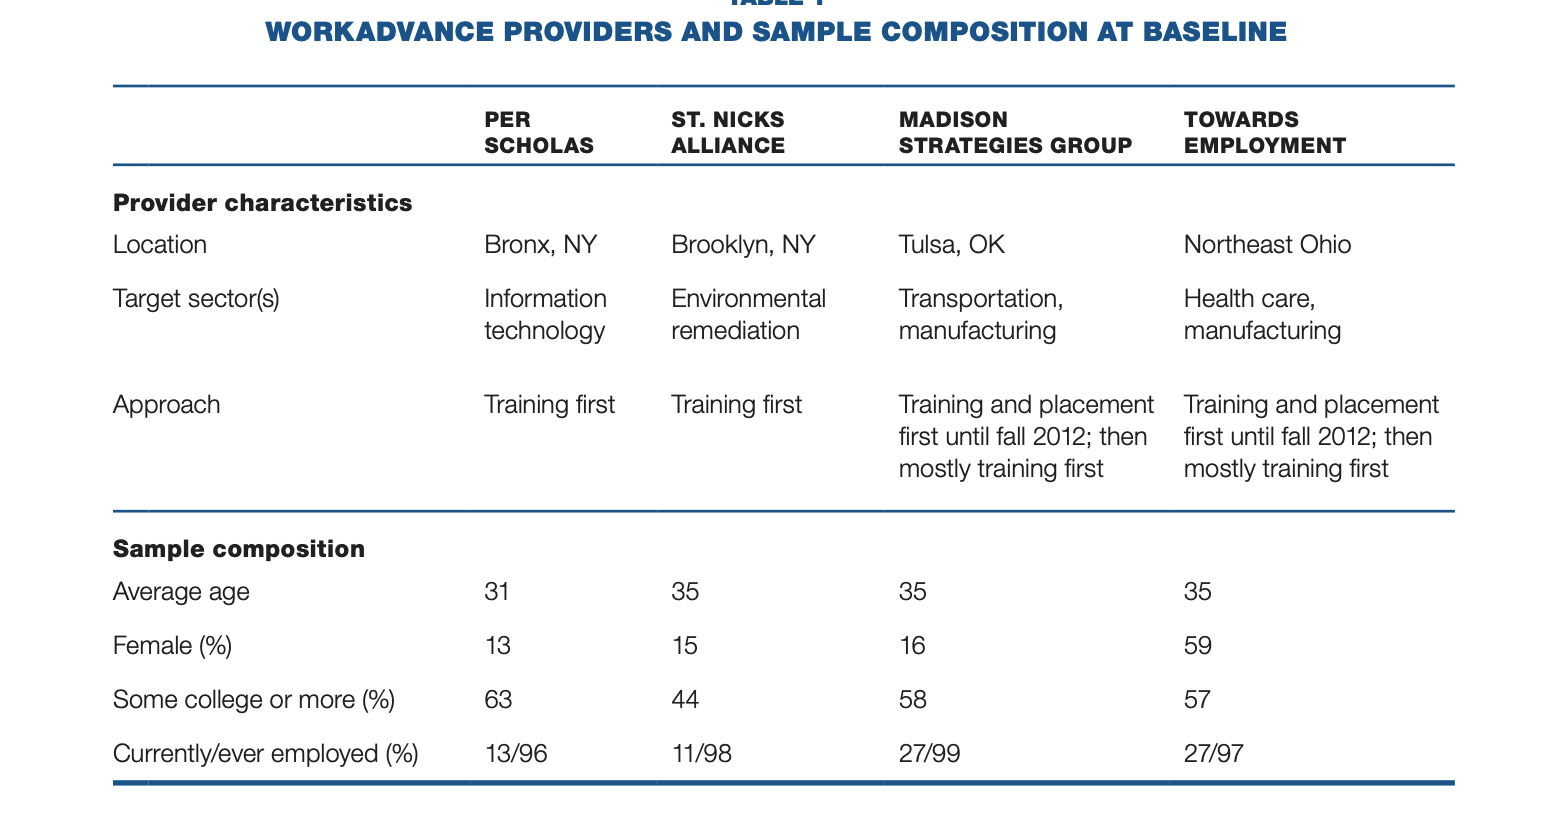
\includegraphics[width = 0.95 \linewidth]{workadvance-site-overview}
\end{frame}


\begin{frame}
\begin{wideitemize}
	\item
	Estimate OLS regression:
	
	$$ \underbrace{Y_i}_{\text{Earnings 2-3 years later}} = \alpha + \beta \underbrace{D_i}_{\text{Treatment indicator}} + \epsilon_i $$
	
	\pause
	\item
	
	\begin{tabular}{lrr}
	Coefficient & Estimate & SE \\
	$\hat\alpha$ & 14636 & 425 \\
	$\hat\beta$ & 1965 & 609
	\end{tabular}
	
	\pause
	\item
	What is the estimated treatment effect? \pause $\hat\beta = 1965$
	
	\item
	What is a CI for the treatment effects? \pause $\hat\beta \pm 1.96 \times SE_{\beta} = \pause{} 1965 \pm 1.96 \times 609 \pause{}  =  [771,3159]$
	
	
	\item
	What is the estimated control mean? \pause $\hat\alpha = 14636$
	
\end{wideitemize}	
	
\end{frame}



\begin{frame}{Roadmap}
	\begin{wideitemize}
		\item \textbf{What we know how to do:} Estimate and test hypotheses about population means using sample means
		\item \textbf{What we want to do:} Estimate approximations to the CEF and test hypotheses about them 
	\end{wideitemize}
	\bigskip
	How can we use what know to do what we want? 
	
	\begin{wideitemize}
		\item 1) Assume the CEF takes a particular form, e.g. linear:
		$$E[Y_i | X_i = x] = \alpha + x \beta \hspace{2cm }\checkmark$$
		
		\item 2) Show that under this assumption, $\alpha$ and $\beta$ can be represented as functions of population means. $\checkmark$
		
		\item
		3) Use our tools for estimating population means using sample means to estimate $\alpha,\beta$ and test hypotheses about them. $\checkmark$
		
		\item
		4) Argue that even if our assumption about the form of the CEF is wrong, the parameters $\alpha,\beta$ may provide a ``good'' approximation.
	\end{wideitemize}
	
\end{frame}



\begin{frame}{Regressions as Approximations}
	\begin{wideitemize}
	\item
	So far we've assumed that the conditional expectation is linear: $E[Y_i | X_i = x]  = \alpha + \beta x$
	
	\item
	What if the true CEF is not linear?!
	
	\pause
	\item
	Claim: if CEF is not linear, then OLS still gives us the ``best linear approximation'' to the CEF 
	\pause 
	\item
	 What we mean by this is that the $\alpha,\beta$ of OLS minimize
	 
	 $$min_{\alpha,\beta} E[ (E[Y|X]  - (\alpha + \beta X) )^2 ]$$
	 
	 \pause
	 That is, we get the linear function that's ``closest'' to the CEF in terms of mean-squared error
	\end{wideitemize}
\end{frame}


\begin{frame}
		
	\begin{center}
		\hspace{0.7cm}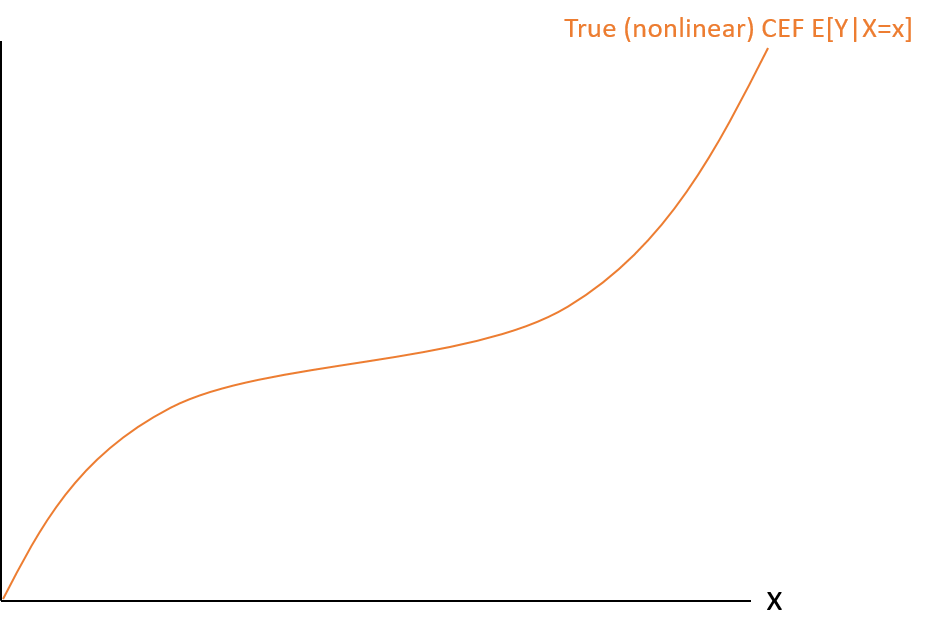
\includegraphics[scale=0.7]{ols1.png}
	\end{center}
	
\end{frame}

\begin{frame}
	
	\begin{center}
		\hspace{0.7cm}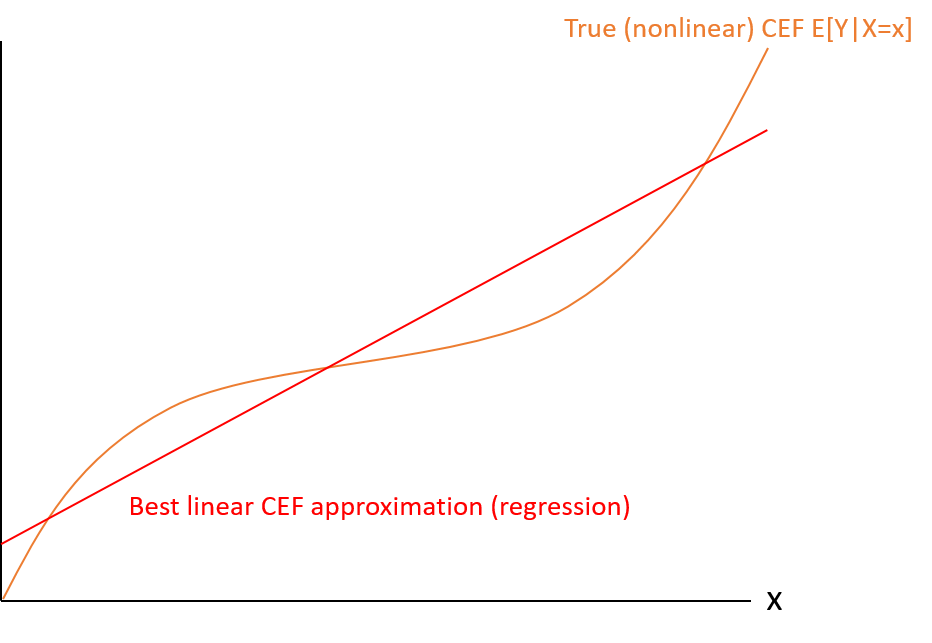
\includegraphics[scale=0.7]{ols2.png}
	\end{center}
	
\end{frame}

\begin{frame}
	
	\begin{center}
		\hspace{0.7cm}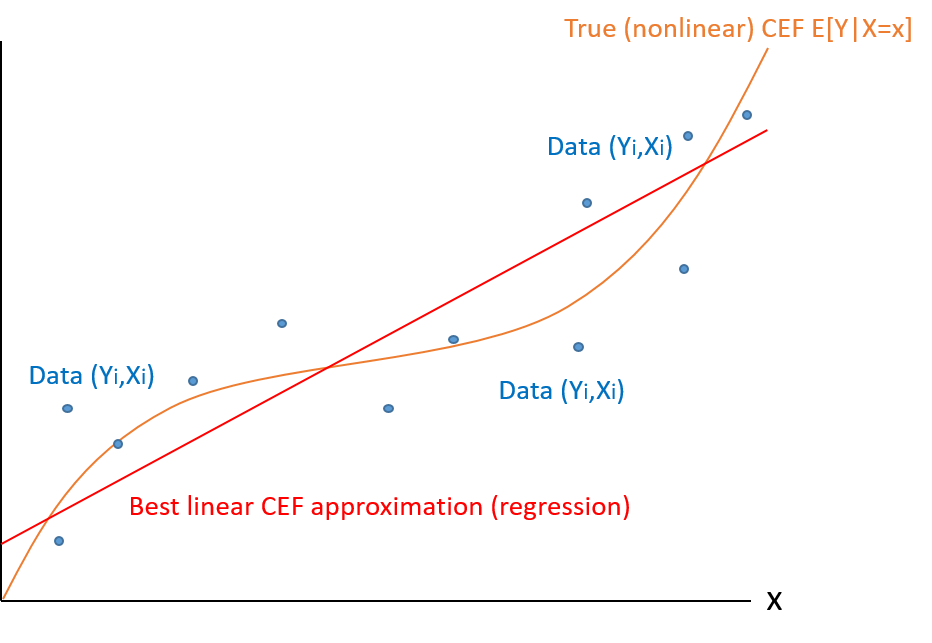
\includegraphics[scale=0.7]{ols3.png}
	\end{center}
	
\end{frame}

\begin{frame}
	
	\begin{center}
		\hspace{0.7cm}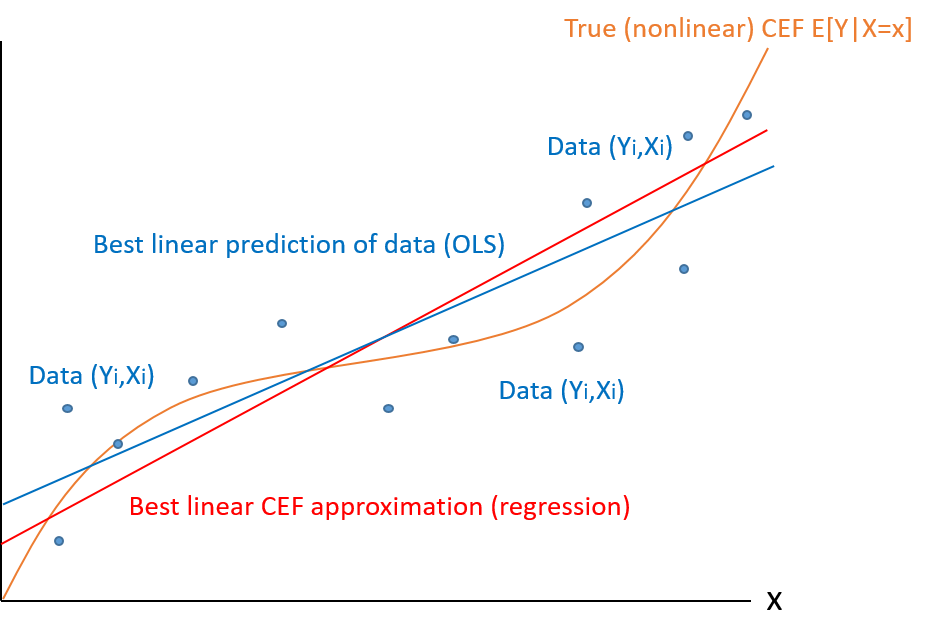
\includegraphics[scale=0.7]{ols4.png}
	\end{center}
	
\end{frame}





\begin{frame}{Proof of OLS as Best Approximation}
	\begin{wideitemize}
		\item 
		We solved for the $\alpha,\beta$ to minimize $E[  (Y - (\alpha + \beta X))^2 ]$.
		
		\pause
		\item
		Let $\mu(x) = E[Y|X=x]$. Then we have \pause
		\begin{align*}
			E[  (Y - (\alpha + \beta X))^2 ]  &= E[ (Y - \mu(X) + \mu(X) -  (\alpha + \beta X))^2   ] \pause{} \\
			&= E[ (Y - \mu(X) )^2 ] + E[(\mu(X) -  (\alpha + \beta X))^2   ]   \\ &+ 2E[ (Y- \mu(X)) (\mu(X)- (\alpha + \beta X))  ]
		\end{align*}
		
		\pause
		\item
		By the LIE, 
		\begin{align*}
			&E[ (Y- \mu(X)) (\mu(X)-(\alpha + \beta X))  ] = \pause{} \\& E[  E[(Y- \mu(X)) (\mu(X)-(\alpha + \beta X)) |X ]    ] = \pause{}\\
			&E[(\mu(X)-(\alpha + \beta X))  \underbrace{ E[Y- \mu(X) | X] }_{=0}] = 0
		\end{align*} 
		
		\item
		Hence, $E[  (Y - (\alpha + \beta X))^2 ] = [ (Y - \mu(X) )^2 ] + E[\mu(X) -  (\alpha + \beta X))^2   ] .$
		
		\noindent But the first term doesn't depend on $\beta$. So minimizing $E[  (Y - (\alpha + \beta X))^2 ]$ is the same as minimizing $E[\mu(X) -  (\alpha + \beta X))^2   ]$
		
	\end{wideitemize}
\end{frame}

\begin{frame}
	\centering
	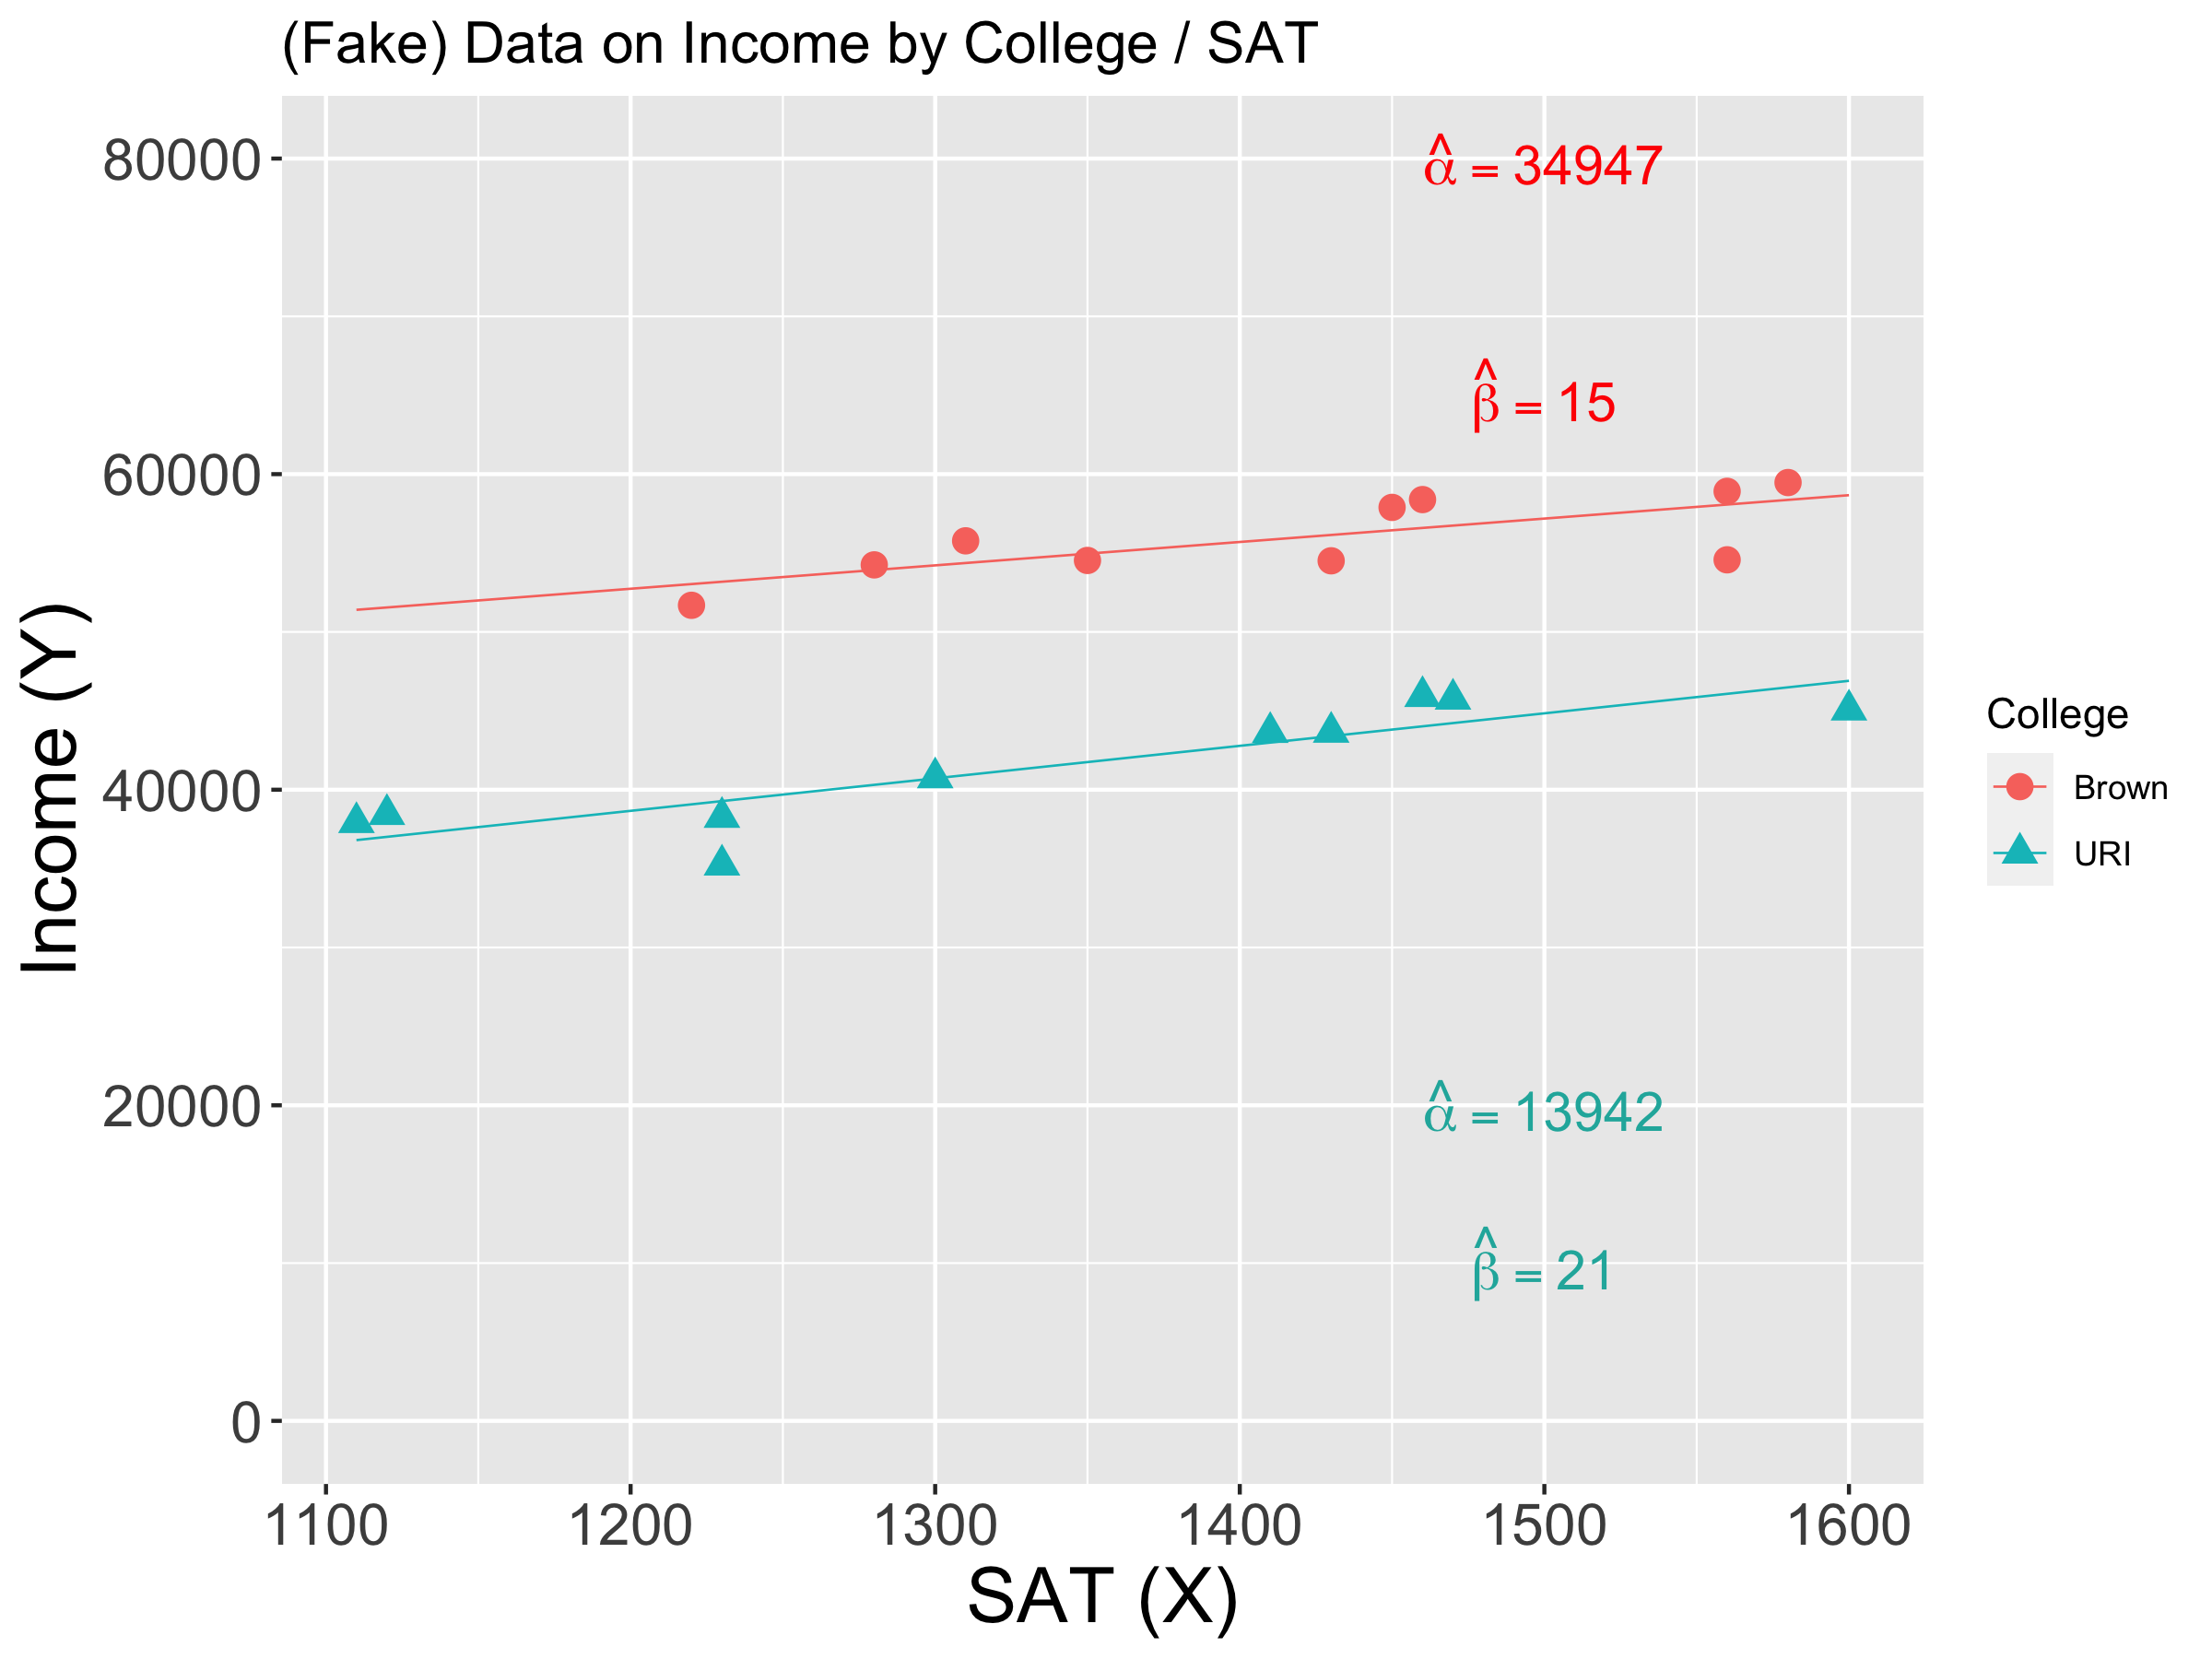
\includegraphics[width =.8\linewidth]{fake-sat-with-trend-both-betas.png}
	
	\begin{wideitemize}
		\item
		 $E[Y_i | D_i = 1, X_i = x]-E[Y_i | D_i = 0, X_i = x]\approx \alpha_1+\beta_1 x - (\alpha_0 +\beta_0x)$; \pause{} $\hat\alpha_1+\hat\beta_1 x - (\hat\alpha_0 +\hat\beta_0x) = (34,947+15 x)-(13,942+21 x)= 21,005-6x$\pause{}
		\item So w/conditional ignorability, $ATE= E[CATE(X_i)]\approx 21,005-6E[X_i]$
	\end{wideitemize}
\end{frame}


		
\end{document}


